\documentclass[a4paper,10pt]{scrreprt}
\usepackage[top=2cm,bottom=2cm,left=2cm,right=2cm]{geometry}
\usepackage[utf8]{inputenc}
\usepackage{graphicx}
\usepackage[german]{babel}
\usepackage{pdfpages}
%opening
\title{Enterprise Application Frameworks}
\author{Florian Thiévent, Roger Kreienbühl}
\usepackage{fancyhdr}
\renewcommand{\familydefault}{\sfdefault}
\newcommand{\pic}[2][figure]{\begin{figure}[h]
 \centering
 \includegraphics[scale=0.3]{#2}
 % rsc.png: 0x0 pixel, 0dpi, 0.00x0.00 cm, bb=
 \caption{#1}
\end{figure}
}
\usepackage{framed}
% Code listenings
\usepackage{color}
\usepackage{xcolor}
\usepackage{listings}
\usepackage{caption}
\DeclareCaptionFont{white}{\color{white}}
\DeclareCaptionFormat{listing}{\colorbox{gray}{\parbox{\textwidth}{#1#2#3}}}
\captionsetup[lstlisting]{format=listing,labelfont=white,textfont=white}
\lstset{
 language=Java,
 basicstyle=\footnotesize\ttfamily, % Standardschrift
 numbers=left,               % Ort der Zeilennummern
 numberstyle=\tiny,          % Stil der Zeilennummern
 stepnumber=5,              % Abstand zwischen den Zeilennummern
 numbersep=5pt,              % Abstand der Nummern zum Text
 tabsize=2,                  % Groesse von Tabs
 extendedchars=true,         %
 breaklines=true,            % Zeilen werden Umgebrochen
 frame=b,         
 %commentstyle=\itshape\color{LightLime}, Was isch das? O_o
 %keywordstyle=\bfseries\color{DarkPurple}, und das O_o
 basicstyle=\footnotesize\ttfamily,
 stringstyle=\color[RGB]{42,0,255}\ttfamily, % Farbe der String
 keywordstyle=\color[RGB]{127,0,85}\ttfamily, % Farbe der Keywords
 commentstyle=\color[RGB]{63,127,95}\ttfamily, % Farbe des Kommentars
 showspaces=false,           % Leerzeichen anzeigen ?
 showtabs=false,             % Tabs anzeigen ?
 xleftmargin=17pt,
 framexleftmargin=17pt,
 framexrightmargin=5pt,
 framexbottommargin=4pt,
 showstringspaces=false      % Leerzeichen in Strings anzeigen ?        
}

\begin{document}

\maketitle
\tableofcontents
\newpage
 \pagestyle{fancy}
\part{Theorie}
\chapter{Einführung in Spring Framework}
\begin{description}
 \item [Dependancy Injection] Den Objekten werden die benötigten Ressourcen und Objekte
zugewiesen. Sie müssen sie nicht selbst suchen.
 
 Wann werden Abhängigkeiten nötig? Der Begriff Dependency Injection (DI) bezeichnet ein Umsetzungsparadigma, das in der objektorientierten Programmierung Anwendung findet.
Dieses Paradigma beschreibt die Arbeitsweise von Frameworks: eine Funktion eines
Anwendungsprogramms wird bei einer Standardbibliothek registriert und von dieser zu einem
späteren Zeitpunkt aufgerufen. Das wird manchmal als eine Anwendung des Hollywood-Prinzips
bezeichnet:don't call us, we'll call you (zu Deutsch: Rufen Sie uns nicht an, wir werden Sie
anrufen): Statt dass die Anwendung den Kontrollfluss steuert und lediglich Standardfunktionen
benutzt, wird die Steuerung der Ausführung bestimmter Unterprogramme an das Framework
abgegeben
\item [Aspect Orientated Programmierung] (AOP): Dadurch kann man vor allem technische Aspekte
wie Transaktionen oder Sicherheit isolieren und den eigentlichen Code davon frei halten.
 

Spring unterstützt die aspektorientierte Programmierung (AOP). AOP ist ein
Programmierparadigma, um verschiedene logische Aspekte eines Anwendungsprogramms (kurz
Anwendung) getrennt voneinander zu entwerfen, zu entwickeln und zu testen. Die getrennt
entwickelten Aspekte werden dann zur endgültigen Anwendung zusammengefügt. In Enterprise
Applikationen werden mit AOP vor allem System Services, wie Transaktion, Sicherheit, ... von der
Business Logik entkoppelt, so dass sich der Programmierer beim Erstellen des Business Objekte
vollkommen auf die Geschäftslogik und dadurch auf den eigentlichen Verwendungszweck der
Applikation konzentrieren kann
\item [Container] Spring ist ein Container, d.h. er enthält und verwaltet den Lebenszyklus und die
Konfiguration von Java-Objekten. Die Java-Objekte sind sogenannte POJOs (Plain-Old-Java-
Objects). Der Spring Container kann schnell herunter- und hinaufgefahren werden. Das ermöglicht
eine effiziente Entwicklung und einen gezielten Einsatz für Unit.Tests. Der Spring Container kann
beispielsweise explizit für einen Unit-Test hochgefahren werden. Der Container kann problemlos im
Java EE, Java SE und in Webapplikationen integriert werden. Auch setzt er keine spezielle
Architektur voraus und benötigt keine umgebungsspezifischen Konfigurationsdateien. Spring wird
einfach mit einer entsprechenden Applikation mitgeliefert.
\item [Framework] Spring erlaubt es eine komplexe Applikation aus einfacheren Komponenten
zusammenzubauen. Das Spring Framework stellt dabei System Services wie
Transaktionsmanagement, Persistenzframework, etc. zur Verfügung, so dass sich der Entwickler
möglichst auf die Business Logik konzentrieren kann.
\item [Vorlagen] (Templates) dienen dazu, die Arbeit mit einigen Programmierschnittstellen (APIs) zu
vereinfachen, indem Ressourcen automatisch aufgeräumt sowie Fehlersituationen einheitlich
behandelt werden.

\end{description}

\begin{figure}[h]
 \centering
 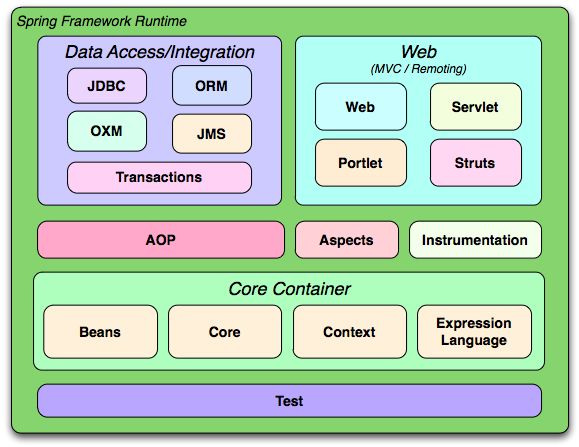
\includegraphics[scale=0.4,keepaspectratio=true]{./spring_framework.png}
 % spring_framework.png: 579x447 pixel, 72dpi, 20.43x15.77 cm, bb=0 0 579 447
\end{figure}


\section{Classpath (Spring HelloWorld) }
\begin{itemize}
 \item JRE + MAVEN + Projekt
 \item \begin{verbatim}
        src/main/java , src/main/res, src/test/java src/test/res 
       \end{verbatim}
 \item kann es auch Buildpath nennen.

\end{itemize}


\begin{verbatim}
localRepository setzen. Nutzt man in STS das Maven-Plugin müssen die entsprechenden
Einstellungen in der Konfiguration des Plugins vorgenommen werden.
<settings xmlns="http://maven.apache.org/SETTINGS/1.0.0"
xmlns:xsi="http://www.w3.org/2001/XMLSchema-instance"
xsi:schemaLocation="http://maven.apache.org/SETTINGS/1.0.0
http://maven.apache.org/xsd/settings-1.0.0.xsd">
<localRepository>d:/projects-dev/repository</localRepository>
</settings>
Listing 1: Eintrag in Maven File settings.xml um lokal den Ort des Repo zu setzen
 
\end{verbatim}

\section{Einfache Entkoppelung mittels Dependancy Injection}
\pic[Herleitung]{herleitung.png}
\subsection{Ausgangspunkt}
\begin{lstlisting}[caption=Ausgangspunkt]
 public class HelloWorld {
  public static void main(String[] args) {
    System.out.println(”Hello World!");
  }
}
  //Der erste Schritt kann folgendermassen aussehen:
 public class DecoupledHelloWorld {
  public static void main(String[] aargh) {
    MessageRenderer mr = new StandardOutRenderer();
    MessageProvider mp = new HelloWorldProvider();
    mr.setMessageProvider(mp);
    mr.render();
    }
}
\end{lstlisting}

\subsection{Versuch 1}
Das Design kann nun durch den Einsatz des Abstract Factory Design Pattern verbessert werden.
Mit der Factory können die konkreten Implementationen "by name" erzeugt werden, wobei die
Namen über ein Konfigurationsfile festgelegt werden. Hier ein Auszug aus einer möglichen
Implementation:

\begin{lstlisting}[caption="Entkoppelung mit manuelles Setzten von Abhängigkeiten]
 public class DecoupledHelloWorldWithFactory {
  public static void main(String[] aargh) {
  MessageRenderer mr =
  MessageSupportFactory.getInstance().getMessageRenderer();
  MessageProvider mp =
  MessageSupportFactory.getInstance().getMessageProvider();
  mr.setMessageProvider(mp);
  mr.render();
  }
}

private MessageSupportFactory() {
...
// Read configuration file
bundle=ResourceBundle.getBundle("ch.edu.msgConf");
// Get Renderer from the configuration
String rendererClass=bundle.getString("renderer.class");
// Get Provider from the configuration
String providerClass=bundle.getString("provider.class");
try {
renderer=(MessageRenderer)
Class.forName(rendererClass).newInstance();
provider=(MessageProvider)
Class.forName(providerClass).newInstance();
} catch (InstantiationException e) {
//exception handling code
} catch (IllegalAccessException e) {
//exception handling code
} catch (ClassNotFoundException e) {
//exception handling code
}
...
}
\end{lstlisting}

\subsection{Völlig entkoppelt}
Grundsätzlich schöner wäre jedoch folgender Code:
DecoupledHelloWorldWithSpring ist nun Spring Applikation, die über eine sogenannte
BeanFactory das Bean mit dem Namen "renderer" ausliest, um anschliessend auf dieser Instanz die
render() Methode auszuführen.
In der Methode getBeanFactory() ist der Zugriff auf die Spring BeanFactory gekapselt. Sie wird
in unserem Falle folgendermassen aussehen:
In dieser Methode wird die Spring-XMLBeanFactory erzeugt. Diese Factory ist in der
"org.springframework.beans-X.X" jar-Bibliothek abgelegt. Die Factory liest das Spring
Konfigurationsfile "helloConfig.xml" und wird die darin enthaltenen Spring Beans instanziieren und
allfällige Abhängigkeiten über Dependency Injection auflösen.
Das Spring Konfigurationsfile ist zentral und legt die konkreten Implementationen fest, die in der
Applikation genutzt werden sollen. In diesem Beispiel kann es folgendermassen aussehen:

\begin{lstlisting}[caption=Depedancy Injection with Spring]
 public class DecoupledHelloWorldWithSpring {
    public static void main(String[] args) {
      BeanFactory factory = getBeanFactory();
      MessageRenderer mr = (MessageRenderer) factory.getBean("renderer");
      mr.render();
  }
}

private static BeanFactory getBeanFactory() {
XmlBeanFactory factory = new XmlBeanFactory(
new ClassPathResource("/spring/helloConfig.xml"));
return factory;
}


\end{lstlisting}
\begin{lstlisting}[caption=Spring Config Datei,language=xml]
 ?xml version="1.0" encoding="UTF-8"?>
<beans xmlns="http://www.springframework.org/schema/beans"
xmlns:xsi="http://www.w3.org/2001/XMLSchema-instance"
#1
xsi:schemaLocation="http://www.springframework.org/schema/beans
http://www.springframework.org/schema/beans/spring-beans-3.2.xsd">
<bean id="renderer" class="edu.spring.domain.renderer.StandardOutRenderer"> #2
<property name="messageProvider" ref=”provider”/> #3
    </bean> 
<bean id="provider" class="edu.spring.domain.provider.HelloWorldProvider" /> #4
</beans>
\end{lstlisting}

\subsection{Besonderheiten}
 \begin{description}

  \item IDs sind optional im Bean file.
  \item Es ist möglich Beans über Klassennamen zu hohlen. Aber muss eine konkrete Implementation nehmen.
  \item [Circular References] a- b -c in xml file.Funktioniert. \textit{Application Context empfohlen}. Instancen gemacht und dann gesetzt mit Setter.
  Was wenn wir eine Abhängigkeiten mit Injection im Kontruktor? Geht nicht - Arbeitsblatt 3. \textbf{Defaultmässig Injection per Setter gemacht}
 \end{description}
 
\chapter{Spring Konfiguration}

\section{Intro}
\pic[Grundlagen der SpringConfig]{spconfig.png}

Als Spring Container stehen zwei Ausprägungen im Zuentrum :
\begin{description}
 \item [BeanFactory:] ist der Container für die Spring Beans. Er stellt den grundlegenden Mechanismus für die Verwaltung der Beans zur Verfügung.
 \item [ApplicationContext:] Erweitert die BeanFactory mit zusätzlicher Funktionalität:
 \begin{itemize}
  \item AOP Features
  \item Message Resource Handling (Internationalizierung)
  \item Even Publication
 \end{itemize}
Wegen diese Features ist die ApplicationContext vvariante bevorzügt.
\end{description}

Die ApllicationContext ist ein Interface. Es existiert folgende verschiedene Implementationen davon :
\begin{description}
 \item [ClassPathXMLApplicationContext] XML File über Classpath geladen.
 \item [FileSystemXMLApplicationContext] XML File über Dateisystem geladen.
 \item [XmlWebApplicationContext] XML Datei über Web Application Context geladen.
\end{description}

Werte von Bean Properties können in Property-Files ausgelagert werden für zusätzliche Flexibilität.\footnote{Ein Property-File ist einfach ein Key-Value Store : muster.eigenschaft=bla}
Properties sollen \textit{nach Instanzierung von Beans} folgen. Deshalb wird dies in Spring Framework als \textbf{BeanFactoryPostProcessor} eingeführt.
Implementationen davon sind : PropertyOverideConfigurer und PropertyPlaceHolderConfigurer. Wobei das zweite öfter zum Einsatz kommt.

\begin{lstlisting}[language=xml,caption=property-placeholder Eintrag]
 <context:property_placeholder location="classpath:app.properties"/>
\end{lstlisting}

\begin{tabular}{c c}
 Element & Beschreibung  \\ \hline
 Context & Spring Schema \\
 property-placeholder & Spring BeanFactory\\
 location & Attribut \\
 ``..'' & Wert \\
 
\end{tabular}

\begin{lstlisting}[language=xml,caption=Einsatzbeispiele von property-placeholder]
 <bean id="provider"
  class="edu...HelloWorldMessageProvider">
  <property name="message" value="${helloworld.message}"/>
  
  
 <!-- JAVA DB Beispiel Property File --!>
 jdbc.driverClassName=org.hsqldb.jdbcDriver
jdbc.local.url=jdbc:hsqldb:hsql://localhost/build/movierental
jdbc.memory.url=jdbc:hsqldb:mem:movierental
jdbc.standalone.url=jdbc:hsqldb:file:build/movierental
jdbc.url=${jdbc.memory.url}
jdbc.username=sa
jdbc.password=...

\end{lstlisting}

\begin{description}
 \item [Bemerkung] er Konstruktor eines ApplicationContext kann immer auch mehrere Config Locations
verarbeiten. Dies ist wichtig, da damit auch auf der Konfigurationsseite eine Strukturierung z.B.
entlang der Server Layers möglich wird. \footnote{Konstruktor nimmt String Array von xml Dateien}

Die XML-Schema basierte Konfiguration wurde mit Spring 2.0 eingeführt und in den folgenden
Versionen immer weiter ausgebaut. Es ersetzt die DTD Version.

Inzwischen gibt es verschiedene Schemas, um die Konfiguration zu vereinfachen. Es sind dies
util, jee, lang, jms, tx, aop,context, tool, beans. Mehr zu diesen Schemas finden sie im
Appendix C der Spring Reference Documentation.


\end{description}

\section{Setter Injection vs Constructor Injection}

\begin{lstlisting}[language=xml,caption=Die zwei Arten von Injection]
 <bean id="renderer" class="edu.spring.domain.renderer.StandardOutRenderer">
<property name="messageProvider" ref="provider"/>
</bean>
<bean id="provider" class="edu.spring.domain.provider.DummyMessageProvider">
<constructor-arg name="message" value="Dummy Message"/>
</bean>

\end{lstlisting}

\begin{tabular}{|l|p{7cm}|p{7cm}|}
\hline
 \textbf{Variante} & \textbf{Vorteil} & \textbf{Nachteil} \\ \hline
 Setter-Injection & \begin{itemize}
                     \item Optionale Properties einfach gesetzt.
                     \item Leichte Handhabung der Properties.
                    \end{itemize} &
                    \begin{itemize}
                     \item Pflicht Properties mussen mit Required annotiert werden.
                    \end{itemize} \\ \hline
 Constructor-Injection & \begin{itemize}
                          \item Mandatory Properties über Konstruktor setzen
                           \item Keine Intanzen die nicht vollständig initializiert sind
                         \end{itemize}& 
                         \begin{itemize}
                          \item Unübersichtlichen Code mit viele Konstruktor-Argumente.
                         \end{itemize} \\ \hline
\end{tabular}

\section{Konfiguration über XML hinaus}

Traditionell wird ein ApplicationContext über eine XML Datei konfiguriert. Die XML-basierte
Konfiguration ist aber nicht die einzige Möglichkeit den Spring Container zu konfigurieren. Da der
Container komplett vom Format der Metadaten entkoppelt ist, stehen dem Programmierer weitere
Möglichkeiten offen, wie:
\begin{itemize}
 \item Annotationsbasiert : seit 2.5
 \item Javabasiert : seit 3.0
\end{itemize}

\begin{tabular}{|l|p{7cm}|p{7cm}|}
\hline
XML-basiert & \begin{itemize}
               \item Keine Kompilation nach Konf Änderungen notwendig.
               \item XML ist bekannt.
               \item Tool Unterstützung ist vorhanden.
               \item Mit Zentralem XML Datei sind die Beans und Äbhangigkeiten dazwischen einfach ersichtlich
              \end{itemize} &
              \begin{itemize}
               \item Überblick verloren bei grossen Projekten. (Mehrere verschiedene XML files)
               \item Kann unübersichtlich sein mit Implementation und Konfiguration getrennt.
              \end{itemize} \\ \hline
Annotationsbasiert & \begin{itemize}
                      \item Implementation und Konfiguration zusammen, besserer Überblick.
                      \item Keine ``XML Hölle''
                     \end{itemize}&
                     \begin{itemize}
                      \item Konfigurationen sind über alle Klassen vertraut. Ist schwierig den Überblick zu behalten.
                      \item Java Quellcode muss zur Verfügung stehen um Konfigurationsänderungen vorzunehmen
                     \end{itemize} \\ \hline
Javabasiert & \begin{itemize}
               \item Kein XML notwendig.
               \item Implementation und Konfiguration sauber getrennt.
               \item Gute Toolunterstützung. 
              \end{itemize} &
              \begin{itemize}
               \item Konfigurationsänderungen führen zu neue Kompilation der Klasse.
              \end{itemize}
\end{tabular}

\subsection{Implementation von Annotationsbasierte Konfiguration}
\begin{lstlisting}[caption=Annotationsbasierte Konfiguration]
@Component // 1
public class StandardOutRenderer implements MessageRenderer {
  @Autowired
  private MessageProvider messageProvider;
  @Override // 2
  public void setMessageProvider(MessageProvider mp) {
    this.messageProvider = mp;
  }
  @Override
  public void render() {
    System.out.println(messageProvider.getMessage());;
  }
}
\end{lstlisting}

\begin{itemize}
 \item Klasse wird als SpringBean konfiguriert. Ich kann der Bean eine Id geben mit entweder @Qualifier oder @Component(``name'')
 \item Hier wird der BeanProperty gesucht vom Typ MessageProvider. Kann auch hier mehr spezifizieren mit @Qualifier
\end{itemize}
\textbf{Bemerkung:} BeanNameGenerator. Wenn keine Name spezifiziert ist wird automatisch die Klassenname genommen mit folgendem Format:
MyClassName $\rightarrow$ myClassName (ist der Bean ID)

\subsection{Scanning für Annotationen in den Klassen}
\begin{lstlisting}[language=xml,caption=Annotation Scanning aktivieren"]
 <context:annotation-config />
<context:component-scan base-package="edu.spring"/>
\end{lstlisting}
\begin{description}
 \item [context:annotation-config] Annotation unterstützung für Dependancy Injection aktivieren. (Erkennung von @Autowired)
 \item [context:component-scan] Erweitert annotation-config sodass Beans über Annotations deklariert werden können.
\end{description}

\section{Spring + Testing}

\begin{lstlisting}[caption=Testing Example]
@RunWith(SpringJUnit4ClassRunner.class)
@ContextConfiguration({"/spring/helloConfig.xml"})
public class HelloWorldMessageProviderAnnotationTest {
  @Autowired
  private MessageProvider messageProvider;
  @Test
  public void testGetMessage() {
  assertEquals("Hello World!", messageProvider.getMessage());
    }
}
\end{lstlisting}
\begin{description}
 \item [RunWith] Spring Spezifische JUnit Test Runner Class benutzt. Resourcen wie config file sind nur innerhalb des gegebenen Pakets zu finden.
 \item [ContextConfiguration] Angabe des Spring Config files.
\end{description}

\chapter{Datenbank}

\section{Data Acess Object Pattern}
\begin{itemize}
 \item DAO sind benutzt um Encapsulation zu erreichen.
 \item 1 DAO 1 Entity.
 \item Nicht für Transaktion, Session oder Verbindung verantwortlich.
 
\end{itemize}

\begin{lstlisting}[caption=GenericDAO]
public interface GenericDao <T, PK extends Serializable> {
PK create(T newInstance);
  T getById(PK id);
  List<T> getAll();
  void update(T obj);
  void delete(T obj);
}
 
\end{lstlisting}

Separiert Persistenz von Business Logik.
\begin{description}
 \item [Strategy Pattern] Nicht 100\% möglich. DAO beinflusst benutzung - nicht mehr POJO. Object Lifecycles (Managed), JDBC : Explicit Update Opartations.
\end{description}

\subsection{Motivation}
\begin{itemize}
 \item Encapsulation
 \item Testability : DAO leichter bei Mock als hibernate Entity Manager
 \item Vendor unabhängigkeit : Abstrahiert verschiedene Implementationen von den gleichen DAO Typ (Hibernate, JDO) 
\end{itemize}

\textbf{Ausnahme:} Falls Business Logik mehrheitlich aus DB Zugriff besteht, dann nutzt diese Trennung nichts.

\section{Service Layer}
\textbf{Aufgaben:}
\begin{itemize}
 \item Core API für andere Schichten der Applikation : Facade Pattern
 \item Core Business Logik : Besteht aus mehrere Aufrufe an DAOs.
 \subitem Movie züruckgegeben oder Servicemethoden für DAO Methoden.
 \item \begin{quotation}
          Combines methods defined in the DAOs and assembles them to
	  cohesive business methods that define an atomic unit of work
 
       \end{quotation}
\subitem Transaktionale Semantik (CRUD)
\subitem Mit Spring AOP realistiert.
\end{itemize}

\section{JDBC Problems}
Wenn mann Verbindungen offen lässt, hat man evtl. keine Verbindungen mehr.
\begin{lstlisting}[caption=Verbindung offen Beispiel : JDBC]
Connection conn = null;
    try {
      conn = ds.getConnection();
      ...
    } catch(SqlException e) { ... }
    } finally {
    if(conn != null){
    try {
      conn.close();
    } catch (SQLException e) {
    throw new RuntimeException(e);
    }
  }
}
\end{lstlisting}

\section{JDBC Probleme}
Gelöst mit Java 7:
\begin{lstlisting}[caption=Java7 JDBC solution]
 Connection conn = null;
try (Connection conn = ds.getConnection()){
...
} catch(SqlException e) { ... }

public interface AutoCloseable {
void close() throws Exception;
}
\end{lstlisting}

Exceptions thrown while closing the resource may be shadowed by the
exceptions thrown while using the resource.

\subsection{JDBC pure DAO}
\begin{lstlisting}[caption=JDBC DAO]
public Movie getById(Long id) {
  Connection conn = null;
  try {
    conn = ds.getConnection();
    Statement st = conn.createStatement();
    ResultSet rs = st.executeQuery(
    "select * from MOVIES where MOVIE_ID = "+id);
    Movie m = null;
    if(rs.next()) {
    long priceCategory = rs.getLong("PRICECATEGORY_FK");
    m = new Movie(rs.getLong("MOVIE_ID"),
    rs.getString("MOVIE_TITLE"),
    rs.getDate("MOVIE_RELEASEDATE"),
    rs.getBoolean("MOVIE_RENTED"),
    priceCategoryDAO.getById(priceCategory));
    }
  return m;
  } catch (SQLException e) {
    throw new RuntimeException(e);
  }
  finally {
    if(conn != null){
	try {
	  conn.close();
      } catch (SQLException e) {
	  throw new RuntimeException(e);
	}
      }
    }
  }
\end{lstlisting}

\begin{lstlisting}[caption=PureJDBC Java 7]
 public Movie getById(Long id) {
    try (Connection conn = ds.getConnection()){
    Statement st = conn.createStatement();
    ResultSet rs = st.executeQuery(
    "select * from MOVIES where MOVIE_ID = "+id);
    if(rs.next()){
      long priceCategory = rs.getLong("PRICECATEGORY_FK");
      return new Movie(rs.getLong("MOVIE_ID"),
      rs.getString("MOVIE_TITLE"),
      rs.getDate("MOVIE_RELEASEDATE"),
      rs.getBoolean("MOVIE_RENTED"),
      priceCategoryDAO.getById(priceCategory));
      } else { return null;}
    } catch (SQLException e) {
      throw new RuntimeException(e);
    }
 }
\end{lstlisting}
\begin{description}
\item[Probleme:] Schreiben von Portable selbstdokumentierte Code der auf spezifischen Fehler reagiert ist problematisch.
\item[Spring Support:] Template um redundante Code zu reduzieren :\\
\begin{itemize}
 \item DAOs mit DI
 \item Automatische Verbindungsverwaltung (Öffenen und Schliessen von Resourcen)
\end{itemize}
Konvertiert auch Exceptions von Frameworks zu eine Hirachie.
\end{description}


\section{Spring Template Pattern}
\begin{itemize}
 \item Öffnen und Schliessen von Verbindungen
 \item Transaktionsverwaltung
 \item SQL Operationen in try catch Blöcke ausführen.
 \item Transaktion Commit und Rollback
 \item Resourcenverwaltung
 \item Exceptions fangen.
\end{itemize}

\textbf{Template Typen:}
\begin{description}
 \item [JdbcTemplate] Generics, Autoboxing, varargd
 \item [NamedParameterJdbcTemplate] Namedparameter, statt Placeholderargumente. Lesbar, und leichter bei Wartung.
\end{description}

\textbf{Template Erzeugung:}
\pic{jdbc.png}

\begin{lstlisting}[caption=JdbcDaoSupport]
public abstract class JdbcDaoSupport extends DaoSupport {
  private JdbcTemplate jdbcTemplate;
  public final void setDataSource(DataSource dataSource) {
    this.jdbcTemplate = createJdbcTemplate(dataSource);
    initTemplateConfig();
  }
  protected JdbcTemplate createJdbcTemplate(DataSource ds) {
    return new JdbcTemplate(ds);
  }
  public final JdbcTemplate getJdbcTemplate() {
    return this.jdbcTemplate;
  }
    protected void initTemplateConfig() { }
    ...
}
\end{lstlisting}

\subsection{JDBC Template : Query Results}
\begin{lstlisting}[caption=JDBC Query Results]
 public Movie getById(Long id){
    JdbcTemplate template = new JdbcTemplate(getDataSource());
    Map<String, Object> res = template.queryForMap(
    "select * from MOVIES where MOVIE_ID = ?", id);
    long priceCategory = (Long)res.get("PRICECATEGORY_FK");
    Movie m = new Movie(
    (Long)res.get("MOVIE_ID"),
    (String)res.get("MOVIE_TITLE"),
    (java.sql.Timestamp)res.get("MOVIE_RELEASEDATE"),
    ((Boolean)res.get("MOVIE_RENTED"),
    priceCategoryDAO.getById(priceCategory));
    return m;
  }
\end{lstlisting}

\begin{lstlisting}[caption=JDBC Query Results (Named Parameters]
 public Movie getById2(Long id) {
    NamedParameterJdbcTemplate template =
    new NamedParameterJdbcTemplate(getDataSource());
    String query = "select * from MOVIES where MOVIE_ID = :id";
    Map<String, Long> params = new HashMap<>();
    params.put("id", id);
    Map<String, Object> res=template.queryForMap(query, params);
    long priceCategory = (Long)res.get("PRICECATEGORY_FK");
    Movie m = new Movie(
    (Long)res.get("MOVIE_ID"),
    (String)res.get("MOVIE_TITLE"),
    (java.sql.Timestamp)res.get("MOVIE_RELEASEDATE"),
    ((Boolean)res.get("MOVIE_RENTED"),
    priceCategoryDAO.getById(priceCategory));
    return m;
  }
\end{lstlisting}

\subsection{Query Results with Callbacks}
Kopieren von Daten in Maps reicht nicht. Callback Methoden können übergegeben werden die von Template ausgeführt werden.

\begin{description}
 \item [ResultSetExtractor] Hohlt JDBC Result Set: \\
 \begin{verbatim}
  interface ResultSetExtractor<T> {
public T extractData(ResultSet arg0)
throws SQLException, DataAccessException;
}
 \end{verbatim}
Implementationen sollen die ganze Resultset verarbeiten, und diese Resultset nicht schliessen.
\item[RowCallBackHandler] ProcessRow aufgerufen für jede Zeile , Resultät im Context gespeichert.
\begin{verbatim}
 interface RowCallbackHandler {
public void processRow(ResultSet arg0)
throws SQLException;
}

\end{verbatim}
\item[RowMapper] gibt objekt zurück, Query gibt Liste zurück.
\begin{verbatim}
 interface RowMapper<T> {
public T mapRow(ResultSet rs, int rowNum)
throws SQLException
}
\end{verbatim}

\end{description}
\begin{lstlisting}[caption=QueryResults Callback Example JDBC]
 public List<Movie> getByTitle(String name) {
  JdbcTemplate template = getJdbcTemplate();
  return template.query(
    "select * from MOVIES where MOVIE_TITLE = ?",
    new RowMapper<Movie>(){	
  public Movie mapRow(ResultSet rs, int row)
  throws SQLException {
    long priceCategory=rs.getLong("PRICECATEGORY_FK");
  return new Movie(
      rs.getLong("MOVIE_ID"),
      rs.getString("MOVIE_TITLE"),
      rs.getTimestamp("MOVIE_RELEASEDATE"),
      rs.getBoolean("MOVIE_RENTED"),
      priceCategoryDAO.getById(priceCategory));
    }
  },
    name
  );
}
\end{lstlisting}

\subsection{Exception Hirachie}
\pic{exheirachie.png}

\section{Resourcen in Spring}
\begin{description}
 \item [Data Sources] javax.sql.Datasource : getConnection() + getConnection(String username,String password)
\end{description}
\begin{lstlisting}[caption=Sample JDBC Declaration von DataSource,language=xml]
 <bean id="dataSource" class=
"org.springframework.jdbc.datasource.DriverManagerDataSource">
<property name="driverClassName"
value="org.hsqldb.jdbcDriver"/>
<property name="url"
value="jdbc:hsqldb:hsql://localhost/lab-db"/>
<property name="username" value="sa"/>
<property name="password" value=""/>
</bean>
\end{lstlisting}

\begin{description}
 \item [org.sfpringframework.jdbc.datasource.DriverManagerDataSource] No connection pooling, ++unitTesting.
 \item [org.apache.commons.dbcp.BasicDataSource] Jakarta, Connection Pooling von aussere JavaEE containers.
 \item [org.springframework.jndi.JndiObjectFactoryBean] für JNDI Verbindungen.
\end{description}

\begin{lstlisting}[caption=Bean Resources JDBC,language=xml]
 <bean id="userDAO"
class="ch.fhnw.edu.rental.daos.impl.JdbcTemplateUserDAO">
<property name="dataSource" ref="dataSource"/>
<property name="rentalDAO
ref="rentalDAO"/>
<property name="movieByIdSql">
<value>select * from MOVIES where MOVIE_ID = ?</value>
</property>
</bean>
<bean id="dataSource" class =
"org.springframework.jdbc.datasource.DriverManagerDataSource"
p:driverClassName="${jdbc.driverClassName}"
p:url="${jdbc.url}"
p:username="${jdbc.username}"
p:password="${jdbc.password}" />
\end{lstlisting}

\section{Testing : DBUnit}
\begin{lstlisting}[caption=DBUnit Test Data]
 <dataset>
<MOVIES
MOVIE_ID='1'
MOVIE_TITLE='Lord of the Rings'
MOVIE_RENTED='1'
PRICECATEGORY_FK='1'/>
<users user_id='1'
USER_NAME='Keller'
USER_FIRSTNAME ='Marc'/>
\end{lstlisting}

\textbf{IDataSet representiert DataSet}
\begin{lstlisting}
 FileInputStream stream = new FileInputStream ("dataset.xml");
FlatXmlDataSetBuilder builder = new FlatXmlDataSetBuilder();
IDataSet dataSet = builder.build(stream);
\end{lstlisting}
\textbf{IDatabaseConnection ist für Datenbankverbindung}
\begin{lstlisting}
IDatabaseConnection connection = new DatabaseConnection(conn);
DatabaseConfig config = connection.getConfig();
config.setProperty(
DatabaseConfig.PROPERTY_DATATYPE_FACTORY,
new HsqldbDataTypeFactory()
);
\end{lstlisting}
\begin{description}
 \item [DatabaseOperation.xxx.execute(connection, dataSet)] xxx=UPDATE,INSERT,DELETE,DELETE\_ALL,REFRESH,CLEAN\_INSERT = DELETE\_ALL+INSERT
 \item [REFRESH] Refresh oder Daten einfügen in DataSet. Existierende rows nicht geändert. 
 \item [TestUtil] Methode getSpringContext ist dann in SetUp methode für alle Tests.Ruft resetData auf ein DBInitializer Instanz.
\end{description}
\begin{lstlisting}[caption=TestUtil Example DBUnit]
 public class JdbcDbInitializer implements DbInitializer {
    public void resetData(ApplicationContext context)
    throws Exception {
    DataSource dataSource = (DataSource)context.getBean(
    "dataSource");
      Connection dbconn = dataSource.getConnection();
	IDatabaseConnection con = ...
	IDataSet ds = ...
    try {
      DatabaseOperation.CLEAN_INSERT.execute(conn, ds);
    } finally { connection.close(); }
  }
}
\end{lstlisting}

\textbf{DataSource Properties:}
\pic[DataSource Properties DBUnit]{dsp.png}

\section{JPA}
\pic[JPA Intro]{jpa1.png}

\begin{lstlisting}
 @Entity
public class Movie {
@Id
private Long id;
private String title;
private boolean rented;
private Date releaseDate;
protected Movie(){}
public Movie(String title, Date releaseDate){ ... }
public String getTitle(){return title;}
public boolean isRented(){return rented;}
public void setRented(boolean rented){this.rented = rented;}
...
}
\end{lstlisting}

\subsection{Entity Manager}
\begin{lstlisting}[caption=Entity Manager JPA]
 EntityManagerFactory emf =
Persistence.createEntityManagerFactory(persistenceUnit);
EntityManager em = emf.createEntityManager();
Movie m = new Movie("Wall-e",
new GregorianCalendar(2011, 9, 25).getTime());
em.persist(m);
m = em.find(Movie.class, 2211);
m.setRented(true);
\end{lstlisting}

\subsection{Entity Annotations}
\begin{lstlisting}[caption=JPA Annotations for Entities]
 @Entity
@Table(name = "CUSTOMERS")
public class Customer implements Serializable {
@Id
@GeneratedValue(strategy=GenerationType.IDENTITY)
private int id;
private String firstName;
@Column(name="NAME")
private String lastName;
protected Customer(){}
public Customer(String firstName, String lastName){
this.firstName = firstName;
this.lastName = lastName;
// id is not set!
}
public int getId() { return this.id; } // read only
public String getFirstName() { return this.firstName; }
public void setFirstName(String firstName) {
this.firstName = firstName;
}
public String getLastName() { return this.lastName; }
public void setLastName(String lastName) {
this.lastName = lastName;
}
}
\end{lstlisting}

\subsection{Entity Klasse Voraussetzungen}
\begin{itemize}
 \item Entity muss mit @Entity annotiert werden.
 \item Default Konstruktor ohne Argumente, kann auch noch andere haben, aber default muss public oder protected sein.
 \item Contraints:
 \subitem Entity Klasse und methoden mussen nicht final sein.
 \subitem Klasse muss eine ``Top Level'' Klasse sein.
 \subsubitem keine innere Klasse, keine Interface, keine Enum.
\end{itemize}

\subsection{Annotation Definitionen}
\begin{description}
 \item [@Entity] Klassifiziert Klasse als Entity : \begin{verbatim}
                                                    @Target(TYPE) @Retention(RUNTIME)
public @interface Entity {
String name() default "";
}
                                                   \end{verbatim}
Name: Entity nennen in Queries muss keine resevierte Wort aus JP-QL sein.
Unqualified  Name von Entity Klasse.
\item[@Table] Gibt die Tabelle für Entity an : \begin{verbatim}
                                                @Target(TYPE) @Retention(RUNTIME)
public @interface Table {
String name() default "";
String catalog() default "";
String schema() default "";
UniqueConstraint[] uniqueConstaints() default {};
}
                                               \end{verbatim}
\begin{description}
 \item [name] Name der Tabelle
 \item [Catalog] Catalog der Tabelle
  \item [schema] Schema der Tabelle]
  \item [uniqueConstaints] Contraints apllied to generated DDL Tables.
\end{description}
\item [@Column] Kolumne für persistente Eigenschaft (Property)
\begin{verbatim}
 @Target({METHOD,FIELD}) @Retention(RUNTIME)
public @interface Column {
String name() default "";
// name of column
boolean unique() default false;
// is DB column unique
boolean nullable() default true; // is DB column nullable
boolean insertable() default true; // is manipulation with a
// sql insert allowed
boolean updatable() default true;
String columnDefinition() default "";
// e.g. CLOB / BLOB
String table() default "";
// table in which field
// is stored (sec. table)
int length() default 255;
// size for strings
int precision() default 0;
// decimal precsion
int scale() default 0;
// decimal scale
}
\end{verbatim}
Unterstützte Typen: char, short, int, long, byte, float, double, boolean.
Strings,Primitive Wrappers, Big Numericals, Java time types. JDBC time types. Byte und Char Arrays, Beliebige Serializable Types.
Entity types \& Collections of entity types
\item [Single Valued Properities] \begin{verbatim}
– T getProperty()
– void setProperty(T t)
                                  \end{verbatim}
Für Multi-valued persistente Eigenschaften muss T von Collection Set List oder Map sein.
\item[@Enumerated] \begin{verbatim}
                    @Target({METHOD,FIELD}) @Retention(RUNTIME)
public @interface Enumerated {
EnumType value() default "ORDINAL";
}
                   \end{verbatim}
Kann Ordinal oder String.
\item[@Lob] Large Object : \begin{verbatim}
                            @Target({METHOD,FIELD}) @Retention(RUNTIME)
public @interface Lob {
}
                           \end{verbatim}
The Lob type is inferred from the type of the persistent field or property,
and (except for string and character-based types) defaults to Blob.
\item[@Transient] Nicht persistentes Feld.
\item[@Id] Typen für ID sind Primitive,Wrapper Typen oder Arrays davon, und String, Large numerics. Temporal Typen.
Generierung : 
\begin{description}
 \item [Assigned] keine key Generation.
 \item [Identity] Auto Increment
 \item [Sequence] DB Specific.
 \item [Table] PK in Seperate Tabelle.
 
\end{description}
\item [@GeneratedValue] \begin{verbatim}
                         Target({METHOD,FIELD}) @Retention(RUNTIME)
public @interface GeneratedValue {
GenerationType strategy() default AUTO;
String generator() default "";
}
public enum GenerationType {TABLE, SEQUENCE, IDENTITY, AUTO};
                        \end{verbatim}
\item[Primary Key Declaration] Simple : Single persistent field. Marked with @Id. Composite Primary Key : Single persistent field or set thereof. PK Klasse muss definiert werden.
Legacy für ID aus mehrere Kolumnen : @EmbeddedId oder @IdClass
\end{description}

\begin{lstlisting}[caption=Annotationsbeispiel]
 @Entity @Table(name="EMP")
public class Employee {
public enum Type {FULL, PART_TIME};
protected Employee(){}
public Employee(String name, Type type){
this.name = name; this.type = type;
}
@Id @GeneratedValue(strategy=GenerationType.IDENTITY)
long id;
@Enumerated(EnumType.STRING)
@Column(name="EMP_TYPE", nullable=false)
Type type;
@Lob byte[] picture;
String name;
}
\end{lstlisting}



\subsection{JPA Inheritance}
\pic{jpainherit.png}

\subsection{JPA Method and Field Annotations}
 \pic{mfannot.png}
 
\subsection{JPA Entity Manager}
\begin{description}
 \item [Zweck] Verwaltet Entity Instanz Lebenszyklus. Methoden um mit PersistenzKontext zu interagieren.
 \item [Managed Objects] Returned oder an Entity Manager gegeben.
 \item [PersistenzKontext] Set of Managed Objects. Nur eine Instanz von jedem Model.
 \item [Erzeugung] Entity Manager Factory.
 
\end{description}

\pic{emdiag.png}

\begin{lstlisting}[language=xml,caption=JPA Persistence Unit]
 <persistence>
<persistence-unit name="movierental"
transaction-type="RESOURCE_LOCAL">
<class>ch.fhnw.edu.rental.model.Movie</class>
<properties>
<property name="hibernate.connection.driver_class"
value="org.hsqldb.jdbcDriver" />
<property name="hibernate.connection.url"
value="jdbc:hsqldb:hsql://localhost/lab-db" />
<property name="hibernate.connection.username"
value="sa" />
<property name="hibernate.connection.password"
value="" />
</properties>
</persistence-unit>
</persistence>
\end{lstlisting}

Erzeugung von EM:
\begin{lstlisting}[caption=Erzeugung von EM]
 EntityManagerFactory emf =
Persistence.createEntityManagerFactory("movierental");
EntityManager em = emf.createEntityManager();

@PersistenceUnit(name="movierental")
EntityManagerFactory emf = null;
@PersistenceContext(name="movierental")
private EntityManager em;

\end{lstlisting}

\begin{lstlisting}[caption=Entity Manager JPA]
 public interface EntityManager {
public void persist(Object entity);
public <T> T merge(T entity);
public void remove(Object entity);
public <T> T find(Class<T> entityClass, Object primaryKey);
...
public void flush();
public void setFlushMode(FlushModeType flushMode);
public FlushModeType getFlushMode();
public void refresh(Object entity);
public void clear();
public boolean contains(Object entity);
public Query createQuery(String ejbqlString);

}
\end{lstlisting}

\begin{description}
 \item[merge] Gibt neue einzigartige Instanz zurück. Insert Operationen.
 \item[refresh] Zustand von Datenbank züruckgegeben. Änderungen ignoriert.
 \item [flush] Persistence sync. 
 \item [clear] entities detatched, nicht flushed entities ignoriert.
 \item [createQuery] \begin{verbatim}
                      Query q = em.createQuery("from Movie m where m.title = :title");
q.setParameter("title", title);
List movies = q.getResultList();
                     \end{verbatim}

\end{description}

\subsection{Spring und Entity Manager }
\begin{lstlisting}[caption= Spring und JPA]
  <bean id="entityManagerFactory" class =
"org.springframework.orm.jpa.LocalEntityManagerFactoryBean">
<property name="persistenceUnitName" value="movierental" />
</bean>
<!--
Persistence unit is defined in persistence.xml that resides in the
META-INF directory on the class path
LocalContainerEntityManagerFactoryBean
– Allows to control the used datasource and the weaving process
Spring supports JPA annotations for persistence contexts / units if a
PersistenceAnnotationBeanPostProcessor is enabled
--!>
<bean class = "org.springframework.orm.jpa.support.
PersistenceAnnotationBeanPostProcessor" />

\end{lstlisting}
\begin{lstlisting}[caption=Spring Injected DAO JPA]
 public class JpaMovieDAO implements MovieDAO {
@PersistenceContext
private EntityManager em;
public Movie getById(Long id) {
return em.find(Movie.class, id);
}
...
\end{lstlisting}

\subsection{Transactions mit JPA}
em.transaction.begin, em.transaction.commit ohne spring, oder :
\begin{lstlisting}[caption=Spring Transactions AOP JPA,language=xml]
 <bean id="transactionManager"
class="org.springframework.orm.jpa.JpaTransactionManager">
<property name="entityManagerFactory"
ref="entityManagerFactory" />
</bean>
<tx:advice id="txAdvice" transaction-manager="transactionManager">
<tx:attributes>
<tx:method name="*" propagation="REQUIRED"/>
</tx:attributes>
</tx:advice>
<aop:config>
<aop:pointcut id="serviceOperation"
expression="execution(* *..*Service.*(..))" />
<aop:advisor advice-ref="txAdvice"
pointcut-ref="serviceOperation" />
</aop:config>
\end{lstlisting}

\subsection{JPA Associations}
\pic[Relationsmöglichkeiten JPA]{relations.png}

\subsubsection{Cascading}
\begin{description}
\item[ PERSIST] Persist auf alle Objekte.
\item[ REMOVE ] Falls entity entfernt ist, dann sind alle damit asozierte Entitäten auch entfernt.Sollte nur für @OneToOne und @OneToMany gelten.
\item[REFRESH] Falls Entität ``refreshed'' ist, dann sind alle assozierte auch so gemacht.
\item [MERGE] Ist ein Entität managed geworden, (Merged mit Persistence Context) dann sind alle assozierte auch so.
\item [DETACHED] Alle Entitäten die damit assoziert sind weden auch als Detatched betrachtet.
\item [ALL] Selbsterklärend

\end{description}


\subsubsection{FetchType}
\pic[JPA FetchType]{eaf_fetchtype.png}

\subsubsection{OneToOne Unidirectional}
0..1 mehr flexibel als 1..1 - 1..1 = Konstruktorparam.
\pic{1to1.png}

\begin{lstlisting}[language=SQL,caption=OnetoOne SQL]
 CREATE MEMORY TABLE ADDRESS(
ID INTEGER NOT NULL PRIMARY KEY,
CITY VARCHAR(255), STREET VARCHAR(255))
CREATE MEMORY TABLE PERSON(
ID INTEGER NOT NULL PRIMARY KEY,
ADDRESS_ID INTEGER NOT NULL,
CONSTRAINT FK203A7330FF0EDE FOREIGN KEY(ADDRESS_ID)
REFERENCES ADDRESS(ID))
\end{lstlisting}

\begin{lstlisting}[caption=OnetoOne Code Java]
 @Entity
public class Person {
@Id @GeneratedValue(strategy=GenerationType.AUTO)
private int id;
private String name;
@OneToOne
private Address address;
private Person(){}
public Person(String name) { this.name = name; }
public int getId() { return id; }
public Address getAddress() { return address; }
public void setAddress(Address address){
this.address = address;}

}
@Entity
public class Address {
@Id @GeneratedValue(strategy=GenerationType.AUTO)
private int id;
private String street, city;
private int zip;
private Address(){}
public Address(String street, int zip, String city) {
this.street = street; this.city = city; this.zip = zip;
}
public int getId() { return id; }
...
}
em.getTransaction().begin();
Person p = new Person("Dominik");
Address a = new Address("Steinackerstrasse", 5210, "Windisch");
p.setAddress(a);
em.persist(p);
em.persist(a); // Only if persist cascading not defined, order of persist operations not relevant.
em.getTransaction().commit();


@Entity
public class Person {
@Id @GeneratedValue(strategy=GenerationType.AUTO)
private int id;
private String name;
@OneToOne(cascade={CascadeType.PERSIST, CascadeType.REMOVE})
private Address address;
private Person(){}
public Person(String name) { this.name = name; }
public int getId() { return id; }
public Address getAddress() { return address; }
public void setAddress(Address address){this.address=address;}
\end{lstlisting}

\begin{lstlisting}[caption=OneToOne Bidirectional]
 @Entity
public class Address {
@Id @GeneratedValue(strategy=GenerationType.AUTO)
private int id;
private String street, city;
private int zip;
@OneToOne(mappedBy="address")
private Person person;
private Address(){}
public Address(String street, int zip, String city) {
this.street = street; this.city = city; this.zip = zip;
}
public Person getPerson() { return person; }
public void setPerson(Person person) { this.person = person; }
}

em.getTransaction().begin();
Person p = new Person("Dominik");
Address a = new Address("Steinackerstrasse", 5210, "Windisch");
p.setAddress(a);
em.persist(p);
em.flush();
// p = em.find(Person.class, 1);
System.out.println(p.getAddress().getStreet());
System.out.println(p.getAddress().getPerson().getName());
em.getTransaction().commit();

//MARKIERT AUF EINE SEITE NUR, MAPPEDBY
\end{lstlisting}

\subsubsection{OneToMany biderectional}
\pic[JPA OnetoMany]{jpa1n.png}
\begin{lstlisting}[caption=JPA 1 to n]
 @Entity
public class Customer {
@Id @GeneratedValue(strategy=GenerationType.AUTO)
private int id;
// this is the inverse side of the relationship
@OneToMany(mappedBy="customer", cascade=CascadeType.ALL)
private Collection<Order> orders;
public Collection<Order> getOrders() {
return orders;
}
public void setOrders(Collection<Order> orders) {
this.orders = orders;
}
}

@Entity
public class Order {
@Id @GeneratedValue(strategy=GenerationType.AUTO)
private int id;
@ManyToOne
// Order is the owner
private Customer customer;
// of the relationship
public Order(){}
public Customer getCustomer() { return customer; }
public void setCustomer(Customer customer) {
this.customer = customer;
}
public int getId() { return id; }
}

\end{lstlisting}

\begin{lstlisting}[language=sql,caption=JPA 1 to n sql]

create table customer (
ID integer
FIRSTNAME varchar(32)
LASTNAME varchar(32)
);

create table address (
ID integer
CUSTOMER_ID integer
STATUS varchar(4)
PRICE decimal(10,2)
);
\end{lstlisting}

\begin{lstlisting}[caption=OneToMany Bidirectional persist JPA]
 em.getTransaction().begin();
Customer c = new Customer();
Order o1 = new Order();
Order o2 = new Order();
List<Order> orders = new LinkedList<Order>();
orders.add(o1); orders.add(o2);
c.setOrders(orders);
em.persist(c);
em.getTransaction().commit();
\end{lstlisting}

\begin{framed}
 \begin{itemize}
  \item n Seite ist immer Besitzer.
  \item Nur referenzen von Order nach Customer sind persisted.
  \item 2 Orders sind im DB gespeichert (persist)
  \item Assoziationen sind nicht persisted.
 \end{itemize}

\end{framed}


\subsubsection{Many to One}
\begin{lstlisting}[caption=JPA Many to One Rental - User]
 @Entity
public class Rental implements Serializable {
@Id
private int id;
@ManyToOne // Rental is the owner of the relationship
@JoinColumn(name="USER_FK") // optional
private User user;
public Rental(){}
public user getUser() { return user; }
public void setUser (Customer user) {
this.user = user;
}
public int getId() { return id; }
public void setId(int id) { this.id = id; }
}

Entity
public class User implements Serializable {
...
@OneToMany(mappedBy="user")
private Collection<Rental> rentals;
// this is the inverse side of the relationship
public Collection<Rental> getRentals() {
return rentals;
}
public void setRentals(Collection<Rental> rentals) {
this.rentals = rentals;
}
}
\end{lstlisting}

\subsubsection{Many to Many}
\pic{nton.png}
\begin{lstlisting}[caption=nton Test JPA]
 em.getTransaction().begin();
Module m1 = new Module("WebFrameworks", "Luthiger");
Module m2 = new Module("ConcurrentProg", "Gruntz");
Student s1 = new Student("Meier");
Student s2 = new Student("Müller");
em.persist(m1);
// all entities are persisted
em.persist(m2);
em.persist(s1);
em.persist(s2);
Collection<Module> modules = new LinkedList<Module>();
modules.add(m1); modules.add(m2);
Collection<Student> students = new LinkedList<Student>();
students.add(s1); students.add(s2);
s1.setModules(modules);
// (1)
m1.setStudents(students);
// (2)
em.getTransaction().commit();

\end{lstlisting}

\pic[n to n Attributen]{ntonattr.png}

\subsubsection{Entity Relation Richtungen}

\begin{description}
 \item [Unidirectional] Hat eine Besizer Seite.
 \item [Bidirectional] Hat Besitzer- und Invers- Seite.
 \item [Besitzerseite] \begin{description}
                        \item [1 to 1] Besizer hat FK
                        \item [n to 1] n hat FK auf 1.
                        \item [n to n] Beide Seiten möglich, Besitzer verwaltet Aktualisierungen der Beziehung im DB.
                       \end{description}
\item[Mapped By] Inverse gibt Besitzerseite an mittels diese Annotation. Nicht im ManyToOne angegeben. Many Seite auto Besitzer.
\end{description}

\subsubsection{orphanRemoval}
\pic{orphrem.png}

\subsubsection{OrderBy}
\pic{ordby.png}

\subsection{Inheritance with JPA}

\pic{jpa_inh.png}

\subsubsection{Single Table Strategy}
\pic{sts.png}
\begin{lstlisting}
 @Inheritance(strategy=InheritanceType.SINGLE_TABLE)
\end{lstlisting}
\begin{itemize}
 \item Alle Attributen in 1 Tabelle.
 \item Typ gespeichert in eine Discriminator Spalte (DType)
 \begin{verbatim}
  @DiscriminatorColumn(String name, DiscriminatorType type)
 name: Name of the column (default: DTYPE)
 type: Type of the column (STRING, CHAR, INTEGER)
 \end{verbatim}
\item Descriminator spezifizieren mit @DescriminatorValue annotation, default ist nicht qualifizierte Klassenname.
\item \textbf{Alle felder die in subklassen addiert sind mussen nullable sein}
\item \textbf{Foreign Keys can only refer to the base class}
\end{itemize}

\subsubsection{Joined Strategy}
\pic{jts.png}
\begin{itemize}
 \item Eine Tabelle ist für jede Klasse definiert, und PK ist verlinkt.
 \item PK ist eine FK die an Basis Tabelle zeigt.
 \item  \textbf{Vorteile:} Normaliserte Schema, Alle Felder können mit NOT NULL definiert werden. FK beziehung zu 
konkrekte Subklassen möglich.
\item \textbf{Nachteile:} Jede Entität muss über mehrere Tabellen gehen.
\end{itemize}

\subsubsection{Table per Class Strategy}
\pic{tpcs.png}
\begin{itemize}
 \item Eine Tabelle ist für jede nicht abstrakte Klasse definiert. Es beinhaltet alle Attributen von diese Klasse und 
die Basisklasse.
\item \textbf{Vorteile:} Non Null Constraints definierbar. FK Referenzen an konkreten Subklassen möglich aber nicht zu 
Abstrakte Basisklassen.
\item \textbf{Nachteile:} Polymoprphic Abfragen nötig, ID Generator nicht nutzbar. Nicht von Jpa2.0 vorrausgesetzt. 
Hibernate stellt es zur Verfügung.
\end{itemize}

\subsubsection{Non Entity Base Class}
Entitätsklassen können von nicht-domänen Klassen abgeleitet werden welche nicht zur TabellenMapping gehören.
\begin{lstlisting}[caption=Entität Basisklasse]
 @MappedSuperclass
public abstract class UuidEntity {
@Id protected String id;
public UuidEntity() { this.id = UUID.randomUUID().toString(); }
public String getId() { return id; }
public boolean equals(Object x) {
return x instanceof UuidEntity
&& ((UuidEntity)x).id.equals(id);
}
public int hashCode() { return id.hashCode(); }
}
\end{lstlisting}

\subsection{JPA Query Sprache (JPQL)}

\begin{description}
 \item [JPQL] Mnipulieren von DB, von SQL inspiriert aber Abfragen sind direkt über Entitäten und ihre Felder.
 \item [Statements] \begin{verbatim}
                     select_statement ::= select_clause from_clause
[where_clause] [groupby_clause] [having_clause] [orderby_clause]
– update_statement ::= update_clause [where_clause]
– delete_statement ::= delete_clause [where_clause]
                    \end{verbatim}
                    \end{description}

\subsubsection{Typed Query}
\begin{itemize}
\item  Queries are created with the method createQuery on an entity manager
\subitem  em.createQuery(String q)  returns a un-typed query
\subitem em.createQuery(String q, Class<T> c)  returns a typed query
\item  Results:
\subitem  q.getResultList()  static type of result is a list (un-typed or typed)
\subitem  q.getSingleResult()  result of type Object or of the expected type
\subsubitem NoResultException if no entry was found
\subsubitem NonUniqueResultException if several entities were found 
\end{itemize}

\begin{lstlisting}[caption=TypedQuery Example]
 TypedQuery<Movie> q = em.createQuery(
"select m from Movie m where m.title = :title",
Movie.class);
q.setParameter("title", title);
List<Movie> movies = q.getResultList();
\end{lstlisting}
\subsubsection{Named Query}
\begin{lstlisting}[caption=Query auf Entitätsklassen]
@NamedQueries({
@NamedQuery(name="movie.all", query="from Movie"),
@NamedQuery(name="movie.byTitle",
query="select m from Movie m where m.title = :title")
})
class Movie {...}
 
\end{lstlisting}
\begin{lstlisting}[caption=Query auf EntitätsManager]
 TypedQuery<Movie> q = em.createNamedQuery(
"movie.byTitle", Movie.class);
q.setParameter("title", title);
List<Movie> movies = q.getResultList();
\end{lstlisting}

\subsubsection{Select und From}
\pic{sundf.png}

\subsubsection{Where Klausel}
\pic{wherek1.png}
\pic{wherek2.png}

\subsubsection{Functions}
\pic{dbfunc.png}
\pic{agfunc.png}
\subsubsection{Ordering and Paging}
\begin{description}
 \item [Order By Klasel] Gibt Resultät eine Ordnung Asc or desc, desc ist default.
 \item [Range beschränken] \begin{itemize}
                            \item public Query setMaxResults(int maxResult)
\item public Query setFirstResult(int startPosition)
\subitem Start with 0
                           \end{itemize}

\end{description}
\begin{lstlisting}[caption=Order und Paging Beispiel]
 TypedQuery<Movie> q = em.createQuery(
"select m from Movie m order by m.name", Movie.class);
q.setFirstResult(20);
q.setMaxResults(10);
List<Movie> movies = q.getResultList();
\end{lstlisting}
\begin{lstlisting}[caption=Weitere Ordering + Paging]
 TypedQuery<Movie> q = em.createQuery(
"select m from Movie m order by m.name", Movie.class);
q.setFirstResult(20);
q.setMaxResults(10);
List<Movie> movies = q.getResultList();
\end{lstlisting}
H2,Postgres mit Hibernate:
\begin{lstlisting}[language=sql]
 SELECT * FROM Movie movie0_
ORDER BY movie0_.name
LIMIT 10
OFFSET 20
\end{lstlisting}
Mysql mit Hibernate:
\begin{lstlisting}[language=sql]
 SELECT * from Movie movie0_
ORDER BY movie0_.name
LIMIT 20, 10
\end{lstlisting}
\begin{lstlisting}[caption=Weitere Beispiele Order + Paging]
 TypedQuery<Movie> q = em.createQuery(
"select m from Movie m order by m.name", Movie.class);
q.setFirstResult(20);
q.setMaxResults(10);
List<Movie> movies = q.getResultList();
\end{lstlisting}
Oracle:
\begin{lstlisting}[language=sql]
 SELECT * FROM
(
SELECT row_.*, rownum rownum_ from
(
SELECT * FROM Movie movie0_ ORDER BY movie0_.name
) row_
WHERE rownum <= 30
)
WHERE rownum_ > 10
\end{lstlisting}

\subsubsection{Inner Joins}
\pic{ijex.png}
\subsubsection{Outer Joins}
\pic{ojex.png}
\subsubsection{Fetch Joins und Lazy Loading}
\pic{fjll.png}
\subsubsection{Update and Delete}
\begin{itemize}
\item With JPA update and delete operations can be performed without
creating instances
\item Can be applied on one entity only (no joins)
\item  Entities which are loaded in a entity context are not changed  => should be executed in a separate transaction
\end{itemize}
\begin{lstlisting}[caption= Bulk update und Delete]
 Query q = em.createQuery(
"delete from Movie m where m.id > 1000");
int result = q.executeUpdate();
\end{lstlisting}

\chapter{Data Transfer Objects}
\begin{description}
 \item [Detatched Entitäten als DTOs] Problems\\
 \begin{itemize}
  \item Lazy load Exceptions werden geworfen falls Felder die noch nicht geladen sind zugegriffen worden sind.
  \item Accessors die keine Exceptions werfen verletzt Verträge.
   \item Reflection gibt proxies züruck die nicht serialisierbar sind.
  \end{itemize}
\item[Data Transfer Objects] Werden benutzt um daten über Schichten der Applikation hinaus zu transportieren. Nur die 
benötigten Daten der Fordernde Layer werden übergegeben nicht alles. Keine Lazy Loading Überraschungen. Clienten sind 
dann ORM unabhängig.
\end{description}
\begin{lstlisting}[caption= DTO Beispiel]
 public class UserDTO implements Serializable {
private Long id;
private String name;
private String firstName;
private List<Long> rentalIds; // allows to access rentals
// on demand
public UserDTO(Long id, String name, String firstName,
List<Long> rentalIds) {
this.id = id;
this.name = name;
this.firstName = firstName;
this.rentalIds = rentalIds;
}
//Service impl JAVA muss innerhabl Transaktion ausgeführt werden.
public UserDTO getUserDataById(Long id) throws ServiceException {
User u = getUserById(id);
List<Long> rentalIds = new ArrayList<Long>();
for(Rental r : u.getRentals()) rentalIds.add(r.getId());
return new UserDTO(u.getId(), u.getName(), u.getFirstName(),
rentalIds);
}
//Service IMPL JPA
public UserDTO getUserDataById(Long id) { // in JpaDAO
Query q = em.createNamedQuery("user.dataById");
q.setParameter("id", id);
UserDTO dto = (UserDTO)q.getSingleResult();
q = em.createNamedQuery("user.rentalsById");
q.setParameter("id", id);
dto.setRentalIDs((List<Long>)q.getResultList());
return dto;
}
@NamedQuery(name="user.dataById", query=
"SELECT NEW ch.fhnw.edu.services.userservice.model.UserDTO(
u.id, u.name, u.firstName) FROM User u WHERE u.id = :id"),
@NamedQuery(name="user.rentalsById", query=
"SELECT r.id FROM User u, IN(u.rentals) r WHERE u.id = :id")
\end{lstlisting}

\section{Dozer}
\begin{itemize}
 \item Java Bean zu Bean Mapper. Kopiert Daten rekursiv. Kann benutzt werden um DTOs zu Kopieren.
 \item Unterstutzt Einfache PropertyMapping, Komplexe TypMappings, Direktionale Mappings, implicit explicit mapping und 
rekursiv Mapping. Mapping von Collections auch unterstutzt.
\end{itemize}
\begin{lstlisting}[caption=DTO Lösung mit Dozer]
 public UserDTO getUserDataById(Long id) throws ServiceException {
return (UserDTO)mapper.map(getUserById(id), UserDTO.class);
}
Mapper mapper; // to be injected by spring
public void setMapper(Mapper mapper) { this.mapper = mapper; }
\end{lstlisting}
\begin{lstlisting}[language=xml]
 <bean id="Mapper" class="org.dozer.DozerBeanMapper">
<property name="mappingFiles">
<list>
<value>dozer.xml</value>
</list>
</property>
</bean>
<mappings>
<configuration>
<custom-converters>
<converter type="ch.fhnw.edu.util.RentalConverter" >
<class-a>
ch.fhnw.edu.services.rentalservice.model.Rental</class-a>
<class-b>java.lang.Long</class-b>
</converter>
</custom-converters>
</configuration>
<mapping type="one-way">
<class-a>ch.fhnw.edu.services.userservice.model.User</class-a>
<class-b>ch.fhnw.edu.services.userservice.model.UserDTO</class-b>
<field>
<a>rentals</a>
<b>rentalIds</b>
</field>
</mapping>
</mappings>
\end{lstlisting}

\section{Pros Cons}
\begin{description}
 \item [-] Dtos haben gleiche Felder wie Domänenobjekten.
 \item [-] Kopieren von Attributen hin und her.
 \item [+] Löst Lazy Loading Problemen.
 \item[+] Design - Müss gedanken machen über Remote Service Facades. Infos aus meherere Entitäten können in DTO 
kombiniert werden. 
\end{description}


\chapter{Remoting with Spring}
 
Spring gibt Remoting Abstraktionen an.
\textit{Gibt unchecked Remote AccessException ersetzt rmi.RemoteException}
\textbf{Bemerkungen:}
\begin{itemize}
 \item Keine standard Unterstützung für security context Propagieren.
 \item Keine Remote Transactionspropagierung.
 \item \textbf{Keine Thread Safety} selbe Bean Instanz kann von mehrere Threads aufgerufen werden.
 \item Keine Session Verwaltung - alle Klienten teilen das selbe Bean Instanz.
 
\end{itemize}


\section{Spring Service Export mit RMI}
\begin{lstlisting}[caption=Spring Config fuer RMI,language=xml]
 <bean class =
"org.springframework.remoting.rmi.RmiServiceExporter">
<property name="serviceName" value="AccountService"/>
<property name="service" ref="accountService"/>
<property name="serviceInterface"
value="ch.fhnw.edu.bank.AccountService"/>
</bean>
\end{lstlisting}

\begin{itemize}
 \item Interface ist POJI = (Plain old Java Interface)
 \item RMIRegistry wird automatisch gestartet falls registryHost nicht explizit angegeben ist.
\end{itemize}

\begin{lstlisting}[caption=spring rmi configuration optionale Eigenschaften,language=xml]
 <property name="registryPort" value="1099"/>
 <property name="registryHost" value="147.86.3.30"/>
 <property name="servicePort" value="7777"/>

default: 1099
default: localhost
default: 0

\end{lstlisting}

\begin{lstlisting}[caption=Server Code für RMI Export]
 public class Server {
public static void main(String[] args) throws Exception {
new ClassPathXmlApplicationContext("context.xml");
System.out.println("server started");
}
}

\end{lstlisting}
Log output : \begin{verbatim}
              INFO: Looking for RMI registry at port '1099'
INFO: Could not detect RMI registry - creating new one
INFO: Binding service 'AccountService' to RMI registry:
RegistryImpl[UnicastServerRef [liveRef:
[endpoint:[10.211.1.33:1099](local),objID:[0:0:0, 0]]]]
server started
             \end{verbatim}




\section{Benutzung ein RMI Dienst mittels Spring}
\begin{lstlisting}[caption=Spring config File : benutzung,language=xml]
 <bean id = "accountService" class =
"org.springframework.remoting.rmi.RmiProxyFactoryBean">
<property name="serviceUrl"
value="rmi://localhost:1099/AccountService"/>
<property name="serviceInterface"
value="ch.fhnw.edu.bank.AccountService"/>
</bean>
\end{lstlisting}

\section{Remoting Exceptions mit Spring}
\pic[Spring Remoting Exception Heirachy]{sreh.png}

\begin{description}
 \item [Adapter] Serverseitig wird ein Adapter angegeben dass RMI Massstäbe folgt. Leitet Requests weiter an Zielobjekt.
 \item [Proxy RemoteInvocationHandler] Client leitet Requests an RMI Interface weiter und wird Exceptions 
mappen.
\end{description}

$ C \rightarrow P \rightarrow A \rightarrow S$ C = Client P = Proxy A = Adapter S = Service.


\section{Spring Remoting Client Seite (nicht Prüfungsrelevant)}

\begin{lstlisting}[caption=Spring Remoting Client Code]
 import java.rmi.Remote;
import java.rmi.RemoteException;
public interface RmiInvocationHandler extends Remote {
  public String getTargetInterfaceName()
  throws RemoteException;
    public Object invoke(RemoteInvocation invocation)
    throws RemoteException,
    NoSuchMethodException,
    IllegalAccessException,
    InvocationTargetException;
}

// The adapter which is registered by Spring in the RMI-registry implements this interface

public class RemoteInvocation implements Serializable {
  private String methodName;
  private Class[] parameterTypes;
  private Object[] arguments;
  // constructors, getters & setters ommitted
  public Object invoke(Object targetObject)
  throws NoSuchMethodException,
  IllegalAccessException,
  InvocationTargetException {
    Method method = targetObject.getClass().getMethod(this.methodName, this.parameterTypes);
    return method.invoke(targetObject, this.arguments);
  }
}
//Executed on the server by the adapter
\end{lstlisting}



\section{Bemerkungen zum Remoting}
\begin{description}
 \item [Regelmässige Objekte]
 \begin{itemize}
  \item Exportierte Objekten können nicht von regelmässige RMI Klienten benutzt werden.
  \item Exportierte Objekten sind vom RmiInvocationWrapper\_Stub bzw RmiInvocationHandler.
  \item Falls Dienst ein Remote Interface anbietet + Service als ServiceInterface spezifiziert ist bei Export, dann ok für normalle Clients.
 \end{itemize}
\item[Client Interface] Benutzt von Klientseite kann Remote sein, kann weniger Methoden enthalten als Interface angegeben von Server.?
\end{description}

\section{HttpInvokers}
\pic{hpinv.png}
\pic{hesp.png}
\pic{burp.png}

\subsection{Config}
\pic{conf1.png}
\pic{conf2.png}

\chapter{Transaktionen}

\section{Key Design Principles}
\begin{description}
 \item [Separation of Concerns] Teile die applikation in eigenartigen Features auf sodass die so disjunkt sind wie 
möglich.
\item [Single Responsibility Principle] Jede Komponent oder Modul sollte nur für ein gegebenes Feature oder 
Funktionalität verantwortlich sein.
\item [Principle of Least Knowledge] Eine Komponente sollte nicht über die interne Details von anderen Komponenten 
wissen (Law of Demeter) LOD.
\item [Don't Repeat Yourself] Nur eine Komponent per Funktionalität.
\item[Avoid doing design upfront] Vermeiden dass man zu viel von Anfang an in Design investiert, bleib lieber Flexibel.
\item [Composition over Inheritance] Inheritance vermehrt die Abhängigkeit und verhindert Reuse.
\end{description}
\section{Key Architecture Principles}
\begin{description}
 \item [Build to change over Build to Last] Design mit der Idee das man es später anpassen kann aufgrund von neuer 
Requirements.
\item[Modellieren zu Analysieren und Risiken vermeiden] Threat Modellen benutzen und UML.
\item[Models und Views als Kollab Tool] Effiziente Komm von design Prinzipien und Veränderungen sind Kritisch. Models 
und andere Visualisierungen Ausnutzen.
\item [Wichtige Ingeneurentscheidungen identifizieren] Entscheidungen von Architektur das erste mal richtig treffen.
\end{description}
\section{SchichtenSystem}
\pic{schichtensys.png}
\section{Enterprise App Design}
\pic{ccex.png}
Serviceschicht Komponenten bieten andere Klienten und Apps eine möglichkeit an, Businesslogik zuzugrefen und 
Appfunktionalität auszunutzen mittels Messagepassing.
Applikationen müssen oftmals mehere arten von Clients unterstützen : \\
\pic{mca.png}

\subsection{OO Design}
Businesslogik soll eine Netzwerk von relativ kleinen Klassen sein und sollte mit die Konzepten der Domänenmodel 
übereinstimmen.
\begin{framed}
 ... "A Domain Model creates a web of interconnected objects, where
each object represents some meaningful individual, whether as large as a
corporation or as small as a single line on an order form."
\end{framed}
\pic{dmex.png}
\pic[Service Beispiel]{servex.png}

\subsection{Enkapselung}
Muss entschieden was Clients aufrufen können. - Interface von BL.
\begin{description}
 \item [+] Maintainability : Implementierung muss nicht Presentation beeinflussen.
 \item[-] Viel Code.
 \item [Optionen] Pojo Facade oder Domain Model öffentlich machen.
\end{description}

\subsection{POJO Facade}
\pic{pjf.png}
\begin{description}
 \item [+] Entwicklung vereinfacht.
 \item [+] Businesslogik kann auserhalb Container getestet werden.
 \item [+] Deklarative Transaktionen und Sicherheit bevor Präsentationsschicht.
 \item [+] Pojo Facade kann Domain Obj züruckgeben und nicht dtos.
 \item [+] Dependency Injection.
 \item [-] Lazy Loading
 \item [-] Verteilte Transaktionen
\end{description}
\subsection{Exposed Model Pattern}
\pic{exmp.png}
\begin{description}
 \item [+] Leicht zu verstehen.
 \item [+] Leichte Navigation in Präsentationsschicht.
 \item [-] Code
 \item [-] LazyLoading Exception
 \item [-] DB Verwaltung in Präsentationsschicht.
 \item [-] Transaktionen im Präsentationsschicht.
\end{description}

\section{Transaktionengrenzen}
\begin{description}
 \item [Präsentationsschicht] \begin{itemize}
                               \item Servlet filters
                               \item Konsistente ansicht der datenbank
                               \item JTA und lokaltransaktionen unterstützt.
                               \item Buffering overhead nötig für Rollback.
                               \item Präsentationscode ist kompliziert 
                               \item \textbf{Programmatic Transaction Model}
                              \end{itemize}
\item [BusinessSchicht] \begin{itemize}
                         \item Transaktion Interceptors
                          \item Keine Konsistenz in transaktionen, zugriff auf Lazy geladene Objekten ausserhalb eine 
Transkaktion
\item \textbf{Deklarative Transaktionsmodell}
                        \end{itemize}


\end{description}

\section{Warum Transaktionen?}
\begin{itemize}
 \item Mehrere Datenbanksysteme sind zugegriffen worden für 1 Request.
  \item Mehere Datenbankzugriffe innerhalb 1 Request.
  \item Verschiedene verteilte Systeme werden zugegriffen für eine Request.
\end{itemize}

\begin{framed}
 \begin{itemize}
  \item Braucht Korrektheit und Recovery Guarantieen.
  \item Applikationsebene wird extrem kompliziert und Debug wird schwierig.
 \end{itemize}

\end{framed}

\section{ACID}
\begin{description}
  
\item[Atomicity] means that a transaction is considered complete if and only if all of
its operations were performed successfully. If any operation in a transaction
fails, the transaction fails.
\item[Consistency] means that a transaction must transition data from one
   consistent state to another, preserving the data's semantic and referential
  integrity. While applications should always preserve data consistency, many
 databases provide ways to specify integrity and value constraints so that
transactions that attempt to violate consistency will automatically fail.
\item[Isolation] means that any changes made to data by a transaction are invisible
   to other concurrent transactions until the transaction commits. Isolation
  requires that several concurrent transactions must produce the same results
 in the data as those same transactions executed serially, in some
(unspecified) order.
\item[Durability] means that committed updates are permanent. Failures that occur
   after a commit cause no loss of data. Durability also implies that data for all
  committed transactions can be recovered after a system or media failure.

\end{description}

\section{Transaktionsdefinitonen}
\begin{description}
 \item [Propagieren] A transaction attribute controls the scope of a transaction
– Example: When method-B executes, does it run within the scope of the
transaction started by method-A, or does it execute with a new transaction?
\pic{tpr.png}
\item[Isolation] In database systems, isolation is a property that the
changes made by an operation are not visible to other
simultaneous operations on the system until its
completion.
\end{description}

\chapter{Transaktions Strategieen}
\section{Theorie}
\begin{description}
\item[ Konsistenz durch Transaktion] Mit Transaktionen im engeren technischen Sinne ist gemeint, dass mehrere 
Arbeitsschritte zusammengefasst werden und entweder alle ausgeführt werden, oder alle nicht ausgeführt werden
(Alles-oder-nichts-Prinzip). Wenn Geld von einem Konto auf ein anderes gebucht werden soll, dann
darf es nicht vorkommen, dass die Abbuchung vom ersten Konto erfolgreich durchgeführt wird, aber
die Gutschrift auf das zweite Konto fehlschlägt. Transaktionen stellen Konsistenz sicher.
\item[Begin, Commit, Rollback, Transaktionsklammer, LUW] \hfill \\
Transaktionen werden durch ein "Begin"-Kommando gestartet. Konnten die einzelnen Arbeitsschritte
erfolgreich durchgeführt werden, werden sie durch ein "Commit"-Kommando endgültig bestätigt (und
für andere Prozesse sichtbar). Gab es einen Fehler, werden sie durch ein "Rollback"-Kommando
zurückgesetzt. Das Begin-Startkommando und das beendende Commit- bzw. Rollback-Kommando
stellt die so genannte Transaktionsklammer dar. Die Arbeitsschritte innerhalb der Transaktion
werden auch schon mal als LUW (Logical Unit of Work) bezeichnet.

\item[Dirty Read] \hfill \\
Wenn Transaktionen dem "ACID"-Prinzip entsprechen sollen, müssen sie serialisiert nacheinander
durchgeführt werden. Aus Performance-Gründen wird hiervon oft abgewichen und ein niedrigerer
"Transaction Isolation Level" eingestellt. Das kann zu folgenden Fehlern führen:
Dirty Read:
Es können von anderen Transaktionen geschriebene Daten gelesen werden, für
die noch kein "Commit" erfolgte und die eventuell per "Rollback" zurückgesetzt
werden.\\
\pic{dread.png}
\item[Non-repeatable Read (Stale Data):] Während einer laufenden Transaktion können Daten von
anderen Transaktionen geändert und committed werden, so dass in der ersten
Transaktion ein zweites Auslesen zu anderen Daten führt.\\
\pic{nrr.png}
\item[Phantom Read] \hfill \\
Eine erste Transaktion liest über eine "Where-Klausel" eine Liste von
Datensätzen. Eine zweite Transaktion fügt weitere Datensätze hinzu (inkl.
Commit). Wenn die erste Transaktion wieder über die gleiche "Where-Klausel"
Datensätze liest oder bearbeitet, gibt es mehr Datensätze als vorher.\\
\pic{pread.png}
\end{description}

\section{Transaction Isolation Levels}
In Datenbanken können verschiedene so genannte "Transaction Isolation Level" eingestellt werden,
um den besten Kompromiss zwischen Isolation und Performance vorzugeben. Folgende
"Transaction Isolation Level" sind in ANSI-SQL2 definiert:
\begin{description}
\item[Read Uncommitted:] Geringste Isolation, höchste Performance, es können Dirty Reads, Non-
repeatable Reads und Phantom Reads auftreten
\item[Read Committed:] Es gibt keine Dirty Reads mehr, aber es gibt weiterhin Non-repeatable Reads und
Phantom Reads
\item[Repeatable Read:] Keine Dirty Reads und keine Non-repeatable Reads, aber weiterhin Phantom
Reads
\item[Serializable:]Keine Dirty Reads, keine Non-repeatable Reads und keine Phantom Reads,
höchste Isolation, geringste Performance
\end{description}
\begin{framed}
In Spring ist der Isolation Level auf DEFAULT gesetzt. Das bedeutet: Aufgabe der Datenbank - Read Committed in unsere 
Beispiel.
\end{framed}

\section{Transaktionen Propagieren}
In einigen Transaktionsmanagern kann die "Transaction Propagation" pro Methode unterschiedlich
eingestellt werden. Es sind nicht immer alle Einstellungen möglich. Die unterschiedlichen
Einstellungen zur Transaction Propagation bewirken beim Eintritt in die jeweilige Methode
Folgendes:
\begin{description}
\item[Required:] Falls bereits vorher eine Transaktion begonnen wurde, wird sie fortgesetzt. Falls
noch keine Transaktion aktiv ist, wird eine neue gestartet.
RequiresNew: Unabhängig davon, ob bereits eine Transaktion aktiv ist, wird immer eine neue
eigene Transaktion gestartet. Diese Transaktion benötigt ein eigenes Commit bzw.
Rollback. Ein Commit bzw. Rollback in dieser neuen Transaktion führt nicht zum
Commit bzw. Rollback in einer eventuell vorher begonnenen Transaktion.
RequiresNew bedingt keine 'Nested Transaction', sondern ein 'Suspend' der
laufenden Transaktion und Einschieben der Untertransaktion. Unabhängig vom
Ergebnis dieser Untertransaktion wird anschließend mit der übergeordneten
Transaktion fortgefahren.
\item[Supports:]
Falls bereits eine Transaktion aktiv ist, wird sie verwendet. Ansonsten wird keine
Transaktion verwendet.
\item[NotSupported:] Die Methode wird immer ohne Transaktion ausgeführt, auch wenn bereits vorher
eine Transaktion gestartet wurde.
\item[Mandatory:] Es muss bereits eine Transaktion aktiv sein. Sonst wird eine Exception geworfen.
\item[Never:] Es darf keine Transaktion aktiv sein. Sonst wird eine Exception geworfen.
\item[Nested:] Eine geschachtelte Transaktion wird gestartet. Diese Option wird meistens nicht
       unterstützt.
\end{description}

\section{Transaktionen mit Spring}

Um das Transaktionshandling in einer Applikation einzuführen, gibt es im Spring-Umfeld mehrere
Möglichkeiten. Die meistverwendete Variante nutzt die Möglichkeiten der Annotation.
\begin{framed}
WICHTIG: In JPA müssen die meisten Manipulationen an den Entitäten eines PersistenceContext
von einer JPA-Transaktion eingehüllt werden. Das betrifft praktisch alle "schreibenden"
EntityManager-Methoden (persist, flush, remove, merge, lock und refresh).
\end{framed}
\begin{description}

\item[@Transactional Annotation anwenden] Die @Transactional Annotation macht das Transaktionshandling in Spring sehr 
einfach. Es genügt die entsprechenden Methoden mit dieser Annotation zu kennzeichnen und das
Transaktionshandling (Transaktion starten und am Ende der Methode commit aufrufen) wird
automatisch durchgeführt.
\begin{lstlisting}[caption=Transaktional über eine Klasse]
 @Transactional
public interface DAO<T> {
T getById(Long id);
List<T> getAll();
void saveOrUpdate(T t);
void delete(T t);
}
\end{lstlisting}
Voraussetzungen für das korrekte Verhalten sind:
1. Die entsprechenenden Methoden müssen mit @Transactional annotiert und sie müssen
"public" sein.
2. Das Transaktionshandling muss in Spring konfiguriert sein.
\end{description}

\section{Bemerkungen zu Transaktionsstrategie}
\begin{description}
 \item [Configuration] 1. Braucht Klasse Annotation, 2. Braucht richtige Spring Konfiguration: \\
 \begin{lstlisting}[caption=spring config transaction,language=xml]
  <context:component-scan base-package="ch.fhnw.edu.rental"/>
  
   <tx:annotation-driven transaction-manager="txManager"/>
  
	<bean id="txManager" class="org.springframework.orm.jpa.JpaTransactionManager">
		<property name="entityManagerFactory" ref="entityManagerFactory" />
	</bean>
	
	
	<bean
		class="org.springframework.orm.jpa.support.PersistenceAnnotationBeanPostProcessor" />
		
		<bean id="entityManagerFactory"
		class="org.springframework.orm.jpa.LocalContainerEntityManagerFactoryBean"
		p:dataSource-ref="dataSource" p:jpaVendorAdapter-ref="jpaAdapter">
		<property name="jpaProperties">
			<props>
				<prop key="hibernate.hbm2ddl.auto">${hibernate.hbm2ddl.auto}</prop>
				<prop key="hibernate.show_sql">${hibernate.show_sql}</prop>
			</props>
		</property>
	</bean>
 \end{lstlisting}
\item[Beispiel Propagation] \begin{verbatim}
                             @Transactional(propagation=Propagation.MANDATORY)
                            \end{verbatim}
\item[Wo Transactional] Überall nicht, aber sollte in service stattfinden und mit ein LUW passieren. \textbf{Default 
propagation = Required} 
\item[Lesende Transaktionen] Bei DAO Methoden die nur lesen mach propagation=Supports.
\item [Exceptionhandling] Checked = kein Rollback, Entwickler, Runtime = User, rollback.
\end{description}


\chapter{Aspektorientierte Programmierung (AOP)}
\begin{lstlisting}[caption=AOP Config,language=xml]
 <tx:advice id="txAdvice" transaction-manager="txManager">
<tx:attributes>
<tx:method name="get*" propagation="SUPPORTS"/>
<tx:method name="*" propagation="REQUIRED"/>
</tx:attributes>
</tx:advice>
<aop:config>
<aop:pointcut id="serviceOperation"
expression="execution(* *..*Service.*(..))" />
<aop:advisor advice-ref="txAdvice"
pointcut-ref="serviceOperation" />
</aop:config>
\end{lstlisting}

\begin{framed}
 Cross Cutting Code sollte soweit von der Applikation weg abstrahiert werden wie möglich.
 Cross cutting code ist code der sich auf Sicherheit, Komm oder Verwaltung bezieht. Integrierung in BL kann Design und 
Warbarkeit sehr schwierig machen. Frameworks helfen damit.
\end{framed}
\section{Definitionen}
\begin{description}
 \item [Cross Cutting Concern] Verhalten mit Data die über die Schichten hinaus benutzt werden kann. Kann nicht 
lokalisiert/in einen Modul verschoben werden..Sicherheit,Transaktionsmanagement,Tracing.
\end{description}

\pic[AOP Terminologie]{aopterm.png}

\section{Advice Typen}
\begin{description}
\item[Before :] Advice that executes before a join point, but which does not have
the ability to prevent execution flow proceeding to the join point (unless it
throws an exception).
\item [After:] Advice to be executed regardless of the means by which a join point
exits (normal or exceptional return).
\item[After Returning :] Advice to be executed after a join point completes
normally: for example, if a method returns without throwing an exception. An
after returning advice has access to the return value (which it cannot modify),
invoked method, methods arguments and target.
\item[After Throwing :] Advice to be executed if a method exits by throwing an
exception.
\item[Around :] Advice that surrounds a join point such as a method invocation.
This is the most powerful kind of advice. Around advice can perform custom
behavior before and after the method invocation. It is also responsible for
choosing whether to proceed to the join point or to shortcut the advised
method execution by returning its own return value or throwing an exception.
\end{description}

Spring benutzt Dynamische AOP Proxies um Cross cutting Unterstützung anzubieten. Field interception fehlt.

\subsection{AOP Implementierungen}
\begin{description}
 \item [Compile Time] Source Code während kompilieren modifiziert. AspectJ
 \item [Runtime - Byte Injection] Class geladen, Subklasse genierert mit aspects - cgilib.
 \item [Runtime - JDK 1.3 Dynamic Proxy] Proxy Object, same interface intercepts and wraps method calls.
\end{description}

\subsection{Sprig AOP Architecture}
\begin{itemize}
 \item Proxybasiert
 \item ProxyFactory für Advised Instanzen.
  \item Proxyfactory nimmt object + aspects gibt Proxy züruck.
  \item Programmatische Ansatz.
  \item ProxyFactoryBean . Deklarative Proxy Erzeugung.
  \item Spring benutzt JDK Dyn Proxies / cgilib um Proxies zu erzeugen.
  \subitem 1 Interface oder mehr JDK Dyn Proxy
  \subitem Keine Interfaces Cgilib Proxy.
\end{itemize}

\section{AOP Calls}
\pic{aopcall.png}
\begin{framed}
Once the call has finally reached the target all subsequent
calls on the object itself are going to be invoked against
the actual target, and not the proxy.
\end{framed}

\subsection{Programmatische Proxies}
\begin{lstlisting}[caption=JDKProxy]
 ProxyFactory factory = new ProxyFactory(new SimplePojo());
factory.addAdvice(new AfterAdvice());
factory.addInterface(Pojo.class);
Pojo pojo = (Pojo) factory.getProxy();
pojo.foo();
\end{lstlisting}
\begin{lstlisting}[caption=CGIlib Proxy]
 ProxyFactory factory = new ProxyFactory(new SimplePojo());
factory.addAdvice(new AfterAdvice());
factory.setProxyTargetClass(true);
Pojo pojo = (Pojo) factory.getProxy();
pojo.foo();
\end{lstlisting}
\section{AOP Development}
\begin{enumerate}
 \item AOP Model : XML / Annotation - AspectJ Support
 \item Advice : advice logik + type.
 \item Pointcut : Definieren mit Expr Language.
\end{enumerate}

\subsection{Aspect J Expression Language}
\begin{description}
 \item [execution -] for matching method execution join points, this is the primary pointcut designator
you will use when working with Spring AOP
\item [within -] limits matching to join points within certain types (simply the execution of a method
declared within a matching type when using Spring AOP)
\item[this -] limits matching to join points (the execution of methods when using Spring AOP) where the
bean reference (Spring AOP proxy) is an instance of the given type
\item[target -] limits matching to join points (the execution of methods when using Spring AOP) where the
target object (application object being proxied) is an instance of the given type
\item[args -] limits matching to join points (the execution of methods when using Spring AOP) where the
arguments are instances of the given types
\item[@target -] limits matching to join points (the execution of methods when using Spring AOP) where
the class of the executing object has an annotation of the given type
\item[@args -] limits matching to join points (the execution of methods when using Spring AOP) where the
runtime type of the actual arguments passed have annotations of the given type(s)
\item[@within -] limits matching to join points within types that have the given annotation (the execution of
methods declared in types with the given annotation when using Spring AOP)
\item[@annotation -] limits matching to join points where the subject of the join point (method being
executed in Spring AOP) has the given annotation
\end{description}
\pagebreak
\subsection{AspectJ Support Beispiel}
\pic{ajs.png}

\subsection{Enable Aspect J}
\pic{enajs.png}
\subsection{AspectJ DI}
\begin{lstlisting}[caption=Aspect J Depedency Injection]
 @Aspect
@Component
// add <component-scan>
public class TracingAnnotations {
@Autowired
private Statistic statistic;
@Before("execution(* edu.GreetingService.say*())")
public void trace() {
// do something with the statistic bean
}
}
\end{lstlisting}

\section{Vorteile Nachteile}
\begin{itemize}
 \item [+] reduces code.
 \item [+] Wartbarkeit
 \item[+] Flexibel Definitionen - XML / Annotationen.
 \item[-] Tool Support, Ausbildung
 \item [-] Warbarkeit nicht richtig, unvorhersehrbare Verhalten (änderung Methodenname).
 \item [-] Entwickler -- unvorhersehrbare Verhalten - Upgrade von Legacy.
 \item [-] Sicherheitsproblemen - AOP unterstutzt keine Weaving.
\end{itemize}

\section{Spring configuration}
\begin{verbatim}
 <aop:aspectj-autoproxy>
\end{verbatim}



\part{Code, Beispiele Übungen}
\chapter{JPA Complete}
\begin{lstlisting}[caption=Movie]
 package ch.fhnw.edu.rental.model;

import java.io.Serializable;
import java.util.Date;

import javax.persistence.Column;
import javax.persistence.Entity;
import javax.persistence.GeneratedValue;
import javax.persistence.Id;
import javax.persistence.JoinColumn;
import javax.persistence.ManyToOne;
import javax.persistence.NamedQueries;
import javax.persistence.NamedQuery;
import javax.persistence.Table;

@Entity
@Table(name = "movies")
@NamedQueries({
	@NamedQuery(name="movie.all", query="from Movie"),
	@NamedQuery(name="movie.byTitle", query="from Movie m where m.title = :title")
})
public class Movie implements Serializable {
	@Id
	@GeneratedValue
	@Column(name = "movie_id")
	private Long id;
	
	@Column(name = "movie_title")
	private String title;
	
	@Column(name = "movie_rented")
	private boolean rented;
	
	@Column(name = "movie_releasedate")
	private Date releaseDate;
	
	@ManyToOne
	@JoinColumn(name = "pricecategory_fk")
	private PriceCategory priceCategory;

	Movie() { 
		// JPA requires that a default constructor is available
	}

	public Movie(String title, Date releaseDate, PriceCategory priceCategory) throws NullPointerException {
		if ((title == null) || (releaseDate == null) || (priceCategory == null)) {
			throw new NullPointerException("not all input parameters are set!");
		}
		this.title = title;
		this.releaseDate = releaseDate;
		this.priceCategory = priceCategory;
		this.rented = false;
	}
	
	public PriceCategory getPriceCategory() {
		return priceCategory;
	}

	public void setPriceCategory(PriceCategory priceCategory) {
		this.priceCategory = priceCategory;
	}

	public String getTitle() {
		return title;
	}

	public Date getReleaseDate() {
		return releaseDate;
	}

	public boolean isRented() {
		return rented;
	}

	public void setRented(boolean rented) {
		this.rented = rented;
	}

	public Long getId() {
		return id;
	}

	public void setId(Long id) {
		this.id = id;
	}

}

\end{lstlisting}

\begin{lstlisting}[caption=Price Category]
 package ch.fhnw.edu.rental.model;

import java.io.Serializable;

import javax.persistence.Column;
import javax.persistence.DiscriminatorColumn;
import javax.persistence.DiscriminatorValue;
import javax.persistence.Entity;
import javax.persistence.GeneratedValue;
import javax.persistence.Id;
import javax.persistence.Inheritance;
import javax.persistence.InheritanceType;
import javax.persistence.NamedQueries;
import javax.persistence.NamedQuery;
import javax.persistence.Table;

@Entity
@Table(name = "pricecategories")
@Inheritance(strategy = InheritanceType.SINGLE_TABLE)
@DiscriminatorValue("PriceCategory")
@DiscriminatorColumn(name = "pricecategory_type")
@NamedQueries({
	@NamedQuery(name="pricecategory.all", query="from PriceCategory")
})
public abstract class PriceCategory implements Serializable {
	@Id
	@GeneratedValue
	@Column(name = "pricecategory_id")
	private Long id;

	public Long getId() {
		return id;
	}

	public void setId(Long id) {
		this.id = id;
	}

	public abstract double getCharge(int daysRented);

	public int getFrequentRenterPoints(int daysRented) {
		return 1;
	}
}

\end{lstlisting}
\begin{lstlisting}[caption=PriceCategory Type Children]
 package ch.fhnw.edu.rental.model;

import javax.persistence.DiscriminatorValue;
import javax.persistence.Entity;
import javax.persistence.Inheritance;
import javax.persistence.InheritanceType;

@Entity
@Inheritance(strategy = InheritanceType.SINGLE_TABLE)
@DiscriminatorValue("ChildrenPriceCategory")
public class PriceCategoryChildren extends PriceCategory {

	@Override
	public double getCharge(int daysRented) {
		double result = 1.5;
		if (daysRented > 3) {
			result += (daysRented - 3) * 1.5;
		}
		return result;
	}

	@Override
	public String toString() {
		return "Children";
	}
}

\end{lstlisting}
\begin{lstlisting}[caption=Rental]
 package ch.fhnw.edu.rental.model;

import javax.persistence.DiscriminatorValue;
import javax.persistence.Entity;
import javax.persistence.Inheritance;
import javax.persistence.InheritanceType;

@Entity
@Inheritance(strategy = InheritanceType.SINGLE_TABLE)
@DiscriminatorValue("ChildrenPriceCategory")
public class PriceCategoryChildren extends PriceCategory {

	@Override
	public double getCharge(int daysRented) {
		double result = 1.5;
		if (daysRented > 3) {
			result += (daysRented - 3) * 1.5;
		}
		return result;
	}

	@Override
	public String toString() {
		return "Children";
	}
}

\end{lstlisting}
\begin{lstlisting}[caption=Role]
 package ch.fhnw.edu.rental.model;

import javax.persistence.Column;
import javax.persistence.Entity;
import javax.persistence.GeneratedValue;
import javax.persistence.Id;
import javax.persistence.Table;

@Entity
@Table(name = "roles")
public class Role {
	@Id
	@GeneratedValue
	@Column(name = "role_id")
	private Long id;
	
	@Column(name = "role_roleName", unique=true)
	private String roleName;
	
	public Role() {
	}

	public String getRoleName() {
		return roleName;
	}

	public void setRoleName(String roleName) {
		this.roleName = roleName;
	}

	public Long getId() {
		return id;
	}

	protected void setId(Long id) {
		this.id = id;
	}
}

\end{lstlisting}
\begin{lstlisting}[caption=User]
 package ch.fhnw.edu.rental.model;

import javax.persistence.Column;
import javax.persistence.Entity;
import javax.persistence.GeneratedValue;
import javax.persistence.Id;
import javax.persistence.Table;

@Entity
@Table(name = "roles")
public class Role {
	@Id
	@GeneratedValue
	@Column(name = "role_id")
	private Long id;
	
	@Column(name = "role_roleName", unique=true)
	private String roleName;
	
	public Role() {
	}

	public String getRoleName() {
		return roleName;
	}

	public void setRoleName(String roleName) {
		this.roleName = roleName;
	}

	public Long getId() {
		return id;
	}

	protected void setId(Long id) {
		this.id = id;
	}
}

\end{lstlisting}

\section{Services}
\begin{lstlisting}[caption=MovieService]
 package ch.fhnw.edu.rental.services.impl;

import java.util.List;

import org.apache.commons.logging.Log;
import org.apache.commons.logging.LogFactory;
import org.springframework.transaction.annotation.Propagation;
import org.springframework.transaction.annotation.Transactional;

import ch.fhnw.edu.rental.daos.MovieDAO;
import ch.fhnw.edu.rental.daos.PriceCategoryDAO;
import ch.fhnw.edu.rental.daos.impl.ManagedDAO;
import ch.fhnw.edu.rental.model.Movie;
import ch.fhnw.edu.rental.model.PriceCategory;
import ch.fhnw.edu.rental.service.RentalServiceException;
import ch.fhnw.edu.rental.services.MovieService;

@Transactional
public class MovieServiceImpl implements MovieService {
	private Log log = LogFactory.getLog(this.getClass());
	
	private MovieDAO movieDAO;
	private PriceCategoryDAO priceCategoryDAO;


	public void setPriceCategoryDAO(PriceCategoryDAO priceCategoryDAO) {
		this.priceCategoryDAO = priceCategoryDAO;
	}

	public void setMovieDAO(MovieDAO movieDAO) {
		this.movieDAO = movieDAO;
	}

	@Transactional(propagation = Propagation.SUPPORTS)
	public Movie getMovieById(Long id) throws RentalServiceException {
		return movieDAO.getById(id);
	}

	@Transactional(propagation = Propagation.SUPPORTS)
	public List<Movie> getAllMovies() throws RentalServiceException {
		List<Movie> movies = movieDAO.getAll();
		if (log.isDebugEnabled()) {
			log.debug("getAllMovies() done");
		}
		return movies;
	}

	@Transactional(propagation = Propagation.SUPPORTS)
	public List<Movie> getMoviesByTitle(String title) throws RentalServiceException {
		return movieDAO.getByTitle(title);
	}

	public void saveOrUpdateMovie(Movie movie) throws RentalServiceException {
		if (movie == null) {
			throw new RentalServiceException("'movie' parameter is not set!");
		}
		movieDAO.saveOrUpdate(movie);
//		throw new Exception("just for testing");
		if (log.isDebugEnabled()) {
			log.debug("saved or updated movie[" + movie.getId() + "]");
		}
	}


	@SuppressWarnings("unchecked")
	public void deleteMovie(Movie movie) throws RentalServiceException {
		if (movie == null) {
			throw new RentalServiceException("'movie' parameter is not set!");
		}
		if (movie.isRented()) {
			throw new RentalServiceException("movie is still used");
		}

		if(movieDAO instanceof ManagedDAO<?>) {
			movie = ((ManagedDAO<Movie>)movieDAO).manage(movie);
		}

		movieDAO.delete(movie);
		
		if (log.isDebugEnabled()) {
			log.debug("movie[" + movie.getId() + "] deleted");
		}
	}

	public List<PriceCategory> getAllPriceCategories() throws RentalServiceException {
		return priceCategoryDAO.getAll();
	}

}

\end{lstlisting}
\begin{lstlisting}[caption=RentalOverdueService]
 package ch.fhnw.edu.rental.services.impl;

import java.util.Calendar;
import java.util.Date;
import java.util.List;

import javax.mail.internet.MimeMessage;

import org.apache.commons.logging.Log;
import org.apache.commons.logging.LogFactory;
import org.springframework.beans.factory.annotation.Autowired;
import org.springframework.beans.factory.annotation.Value;
import org.springframework.scheduling.annotation.Scheduled;
import org.springframework.stereotype.Component;

import ch.fhnw.edu.rental.model.Rental;
import ch.fhnw.edu.rental.service.RentalServiceException;
import ch.fhnw.edu.rental.services.MailService;
import ch.fhnw.edu.rental.services.RentalOverdueService;
import ch.fhnw.edu.rental.services.RentalService;

@Component("rentalOverdueService")
public class RentalOverdueServiceImpl implements RentalOverdueService  {
	private Log log = LogFactory.getLog(RentalOverdueServiceImpl.class);

	@Autowired
	private RentalService rentalService;
	
	@Autowired
	private MailService mailService;
	
	@Value("${jobs.simulation}")
	private boolean simulation;
	
	@Value("${mail.reminder.template}")
	private String template;

	@Override
	@Scheduled(fixedRate = 10000)
	public void checkRentals() throws RentalServiceException {
		Date today;
		List<Rental> rentals = rentalService.getAllRentals();
		Calendar cal = Calendar.getInstance();
		today = cal.getTime();
		for (Rental rental : rentals) {
			cal.setTime(rental.getRentalDate());
			cal.add(Calendar.DAY_OF_YEAR, rental.getRentalDays());
			Date dueDate = cal.getTime();
			if (today.after(dueDate)) {
				if (! simulation) {
					MimeMessage message = mailService.prepareMailMessage(rental, template);
					mailService.sendMailMessage(message);
					log.info("Reminder for user '" + rental.getUser().getLastName()
							+ " " + rental.getUser().getFirstName()	+ "' sent");
				} else {
					log.debug("Simulation: Reminder for user '" + rental.getUser().getLastName()
							+ " " + rental.getUser().getFirstName()	+ "' sent");
				}
			}
		}
	}
}

\end{lstlisting}
\begin{lstlisting}[caption=MailService]
 package ch.fhnw.edu.rental.services.impl;

import java.util.Map;

import javax.mail.MessagingException;
import javax.mail.internet.MimeMessage;

import org.apache.commons.logging.Log;
import org.apache.commons.logging.LogFactory;
import org.springframework.mail.javamail.JavaMailSender;
import org.springframework.mail.javamail.MimeMessageHelper;
import org.springframework.stereotype.Component;

import ch.fhnw.edu.rental.model.Rental;
import ch.fhnw.edu.rental.service.RentalServiceException;
import ch.fhnw.edu.rental.services.MailService;
import ch.fhnw.edu.rental.services.impl.util.MailModelHelper;
import ch.fhnw.edu.rental.services.impl.util.MailTemplateHelper;

@Component
public class MailServiceImpl implements MailService {
	private Log log = LogFactory.getLog(MailServiceImpl.class);

	private JavaMailSender mailSender;
	private String mailFromAddress;
	private String mailSubject;
	private MailModelHelper mailModelHelper;
	private MailTemplateHelper mailTemplateHelper;

	public void setMailSubject(String mailSubject) {
		this.mailSubject = mailSubject;
	}

	public void setMailFromAddress(String mailFromAddress) {
		this.mailFromAddress = mailFromAddress;
	}

	public void setMailSender(JavaMailSender mailSender) {
		this.mailSender = mailSender;
	}

	public void setMailModelHelper(MailModelHelper mailModelHelper) {
		this.mailModelHelper = mailModelHelper;
	}

	public void setMailTemplateHelper(MailTemplateHelper mailTemplateHelper) {
		this.mailTemplateHelper = mailTemplateHelper;
	}

	@Override
	public MimeMessage prepareMailMessage(final Rental rental, final String template) throws RentalServiceException 
{
		try {
			MimeMessage mimeMessage = mailSender.createMimeMessage();
			MimeMessageHelper helper = new MimeMessageHelper(mimeMessage, "UTF-8");
			helper.setTo(rental.getUser().getEmail());
			helper.setFrom(mailFromAddress);
			helper.setSubject(mailSubject);
			Map<String, Object> model = mailModelHelper.fillModel(rental);
			String textMessage = mailTemplateHelper.mergeTemplate(model, template);
			helper.setText(textMessage);
			log.debug("Mail prepared for '" + rental.getUser().getLastName() + " " + 
rental.getUser().getFirstName());
			return helper.getMimeMessage();
		} catch (MessagingException e) {
			throw new RentalServiceException(e.getMessage());
		}
	}

	@Override
	public void sendMailMessage(MimeMessage message) {
		mailSender.send(message);	
		log.debug("Mail sent successfully");
	}
}

\end{lstlisting}
\begin{lstlisting}[caption=RentalService]
 package ch.fhnw.edu.rental.services.impl;

import java.util.Date;
import java.util.List;

import org.apache.commons.logging.Log;
import org.apache.commons.logging.LogFactory;
import org.springframework.transaction.annotation.Propagation;
import org.springframework.transaction.annotation.Transactional;

import ch.fhnw.edu.rental.daos.MovieDAO;
import ch.fhnw.edu.rental.daos.RentalDAO;
import ch.fhnw.edu.rental.daos.impl.ManagedDAO;
import ch.fhnw.edu.rental.model.Rental;
import ch.fhnw.edu.rental.service.RentalServiceException;
import ch.fhnw.edu.rental.services.RentalService;

@Transactional
public class RentalServiceImpl implements RentalService {
	private Log log = LogFactory.getLog(this.getClass());
	
	private RentalDAO rentalDAO;
	
	public void setRentalDAO(RentalDAO rentalDAO) {
		this.rentalDAO = rentalDAO;
	}

	private MovieDAO movieDAO;
	
	public void setMovieDAO(MovieDAO movieDAO) {
		this.movieDAO = movieDAO;
	}

	@Override
	@Transactional(propagation = Propagation.SUPPORTS)
	public List<Rental> getAllRentals() throws RentalServiceException {
		List<Rental> rentals = rentalDAO.getAll();
		if (log.isDebugEnabled()) {
			log.debug("getAllRentals() done");
		}
		return rentals;
	}

	@Override
	@Transactional(propagation = Propagation.SUPPORTS)
	public int calcRemainingDaysOfRental(Rental rental, Date date) {
		return rental.calcRemainingDaysOfRental(date);
	}

	@Override
	@Transactional(propagation = Propagation.SUPPORTS)
	public Rental getRentalById(Long id) {
		return rentalDAO.getById(id);
	}

	@SuppressWarnings("unchecked")
	@Override
	public void deleteRental(Rental rental) throws RentalServiceException {
		if (rental == null) {
			throw new RentalServiceException("'rental' parameter is not set!");
		}
		if(rentalDAO instanceof ManagedDAO<?>) {
			rental = ((ManagedDAO<Rental>)rentalDAO).manage(rental);
		}

		rental.getUser().getRentals().remove(rental);
		rental.getMovie().setRented(false);

		rentalDAO.delete(rental);
		
		if( !(movieDAO instanceof ManagedDAO<?>)){
			movieDAO.saveOrUpdate(rental.getMovie());
		}
		
		if (log.isDebugEnabled()) {
			log.debug("rental[" + rental.getId() + "] deleted");
		}		
	}
}

\end{lstlisting}
\begin{lstlisting}[caption=UserService]
 package ch.fhnw.edu.rental.services.impl;

import java.util.List;

import org.apache.commons.logging.Log;
import org.apache.commons.logging.LogFactory;
import org.springframework.transaction.annotation.Propagation;
import org.springframework.transaction.annotation.Transactional;

import ch.fhnw.edu.rental.daos.MovieDAO;
import ch.fhnw.edu.rental.daos.RentalDAO;
import ch.fhnw.edu.rental.daos.UserDAO;
import ch.fhnw.edu.rental.daos.impl.ManagedDAO;
import ch.fhnw.edu.rental.model.Movie;
import ch.fhnw.edu.rental.model.Rental;
import ch.fhnw.edu.rental.model.User;
import ch.fhnw.edu.rental.service.RentalServiceException;
import ch.fhnw.edu.rental.services.UserService;

@Transactional
public class UserServiceImpl implements UserService {
	private Log log = LogFactory.getLog(this.getClass());
	
	private UserDAO userDAO;
	private RentalDAO rentalDAO;
	private MovieDAO movieDAO;

	public void setUserDAO(UserDAO userDAO) {
		this.userDAO = userDAO;
	}

	public void setRentalDAO(RentalDAO rentalDAO) {
		this.rentalDAO = rentalDAO;
	}

	public void setMovieDAO(MovieDAO movieDAO) {
		this.movieDAO = movieDAO;
	}

	@Override
	@Transactional(propagation = Propagation.SUPPORTS)	
	public User getUserById(Long id) throws RentalServiceException {
		User user = this.userDAO.getById(id);
		return user;
	}
	
	@Override
	@Transactional(propagation = Propagation.SUPPORTS)	
	public List<User> getAllUsers() throws RentalServiceException {
		List<User> users = userDAO.getAll();
		if (log.isDebugEnabled()) {
			log.debug("getAllUsers() done");
		}
		return users;
	}

	@Override
	public void saveOrUpdateUser(User user) throws RentalServiceException {
		userDAO.saveOrUpdate(user);
		if (log.isDebugEnabled()) {
			log.debug("saved or updated user[" + user.getId() + "]");
		}
	}

	@Override
	@SuppressWarnings("unchecked")
	public void deleteUser(User user) throws RentalServiceException {
		if (user == null) {
			throw new RentalServiceException("'user' parameter is not set!");
		}
		if(userDAO instanceof ManagedDAO<?>) {
			user = ((ManagedDAO<User>)userDAO).manage(user);
		}

		userDAO.delete(user);	// if (user.getRentals().size()>0) associated rentals 
								// have to be deleted by userDAO.delete(user) as well
		if (log.isDebugEnabled()) {
			log.debug("user[" + user.getId() + "] deleted");
		}
	}

	@Override
	@Transactional(propagation = Propagation.SUPPORTS)	
	public List<User> getUsersByName(String name) throws RentalServiceException {
		List<User> users = userDAO.getByName(name);
		return users;
	}

	@Override
	@SuppressWarnings("unchecked")
	public Rental rentMovie(User user, Movie movie, int days)
			throws RentalServiceException {
		if (user == null) 
			throw new IllegalArgumentException("parameter 'user' is null!");
		if (movie == null) 
			throw new IllegalArgumentException("parameter 'movie' is null!");
		if (days < 1)
			throw new IllegalArgumentException("parameter 'days' must be > 0");

		// In case of managed daos, the detached entities are merged first.
		if(movieDAO instanceof ManagedDAO<?>) {
			movie = ((ManagedDAO<Movie>)movieDAO).manage(movie);
		}
		if(userDAO instanceof ManagedDAO<?>) {
			user = ((ManagedDAO<User>)userDAO).manage(user);
		}
		
		Rental rental = new Rental(user, movie, days);
		rentalDAO.saveOrUpdate(rental);
		// the constructor of rental changed the movie to rented, this change must
		// be persisted in case of non managed DAOs.
		if(! (movieDAO instanceof ManagedDAO)){
			movieDAO.saveOrUpdate(movie);
		}
		// Similarly, the user has to be saved as he refers to an additional rental
		// in case that the user is not managed and in case that the user is the 
		// owner of the association.
		// if(! (userDAO instanceof ManagedDAO)) {
		// 	userDAO.saveOrUpdate(user);
		// }
		
		return rental;
	}
	
	@Override
	@SuppressWarnings("unchecked")
	@Transactional(propagation = Propagation.SUPPORTS)	
	public void returnMovie(User user, Movie movie)
			throws RentalServiceException {
		if (user == null) 
			throw new IllegalArgumentException("parameter 'user' is null!");
		if (movie == null) 
			throw new IllegalArgumentException("parameter 'movie' is null!");
		if(userDAO instanceof ManagedDAO<?>) {
			user = ((ManagedDAO<User>)userDAO).manage(user);
		}
		if(movieDAO instanceof ManagedDAO<?>) {
			movie = ((ManagedDAO<Movie>)movieDAO).manage(movie);
		}

		Rental rentalToRemove = null;
		for (Rental rental : user.getRentals()) {
			if (rental.getMovie().equals(movie)) {
				rentalToRemove = rental;
				break;
			}
		}
		
		user.getRentals().remove(rentalToRemove);
		rentalToRemove.getMovie().setRented(false);
		rentalDAO.delete(rentalToRemove);
	}
}

\end{lstlisting}
\chapter{Discussions JPA}
\section{JPA Cascade Types}
The cascade types supported by the Java Persistence Architecture are as below:
\begin{enumerate}
	 
\item  \textbf{CascadeType.PERSIST} : cascade type presist means that save() or persist() operations cascade to related entities.
\item  \textbf{CascadeType.MERGE} : cascade type merge means that related entities are merged when the owning entity is merged.
\item  \textbf{CascadeType.REFRESH} : cascade type refresh does the same thing for the refresh() operation.
\item  \textbf{CascadeType.REMOVE} : cascade type remove removes all related entities association with this setting when the owning entity is deleted.
\item  \textbf{CascadeType.DETACH} : cascade type detach detaches all related entities if a “manual detach” occurs.
\item  \textbf{CascadeType.ALL} : cascade type all is shorthand for all of the above cascade operations.
\end{enumerate}
There is no default cascade type in JPA. By default no operations are cascaded.
\section{JDBC}
 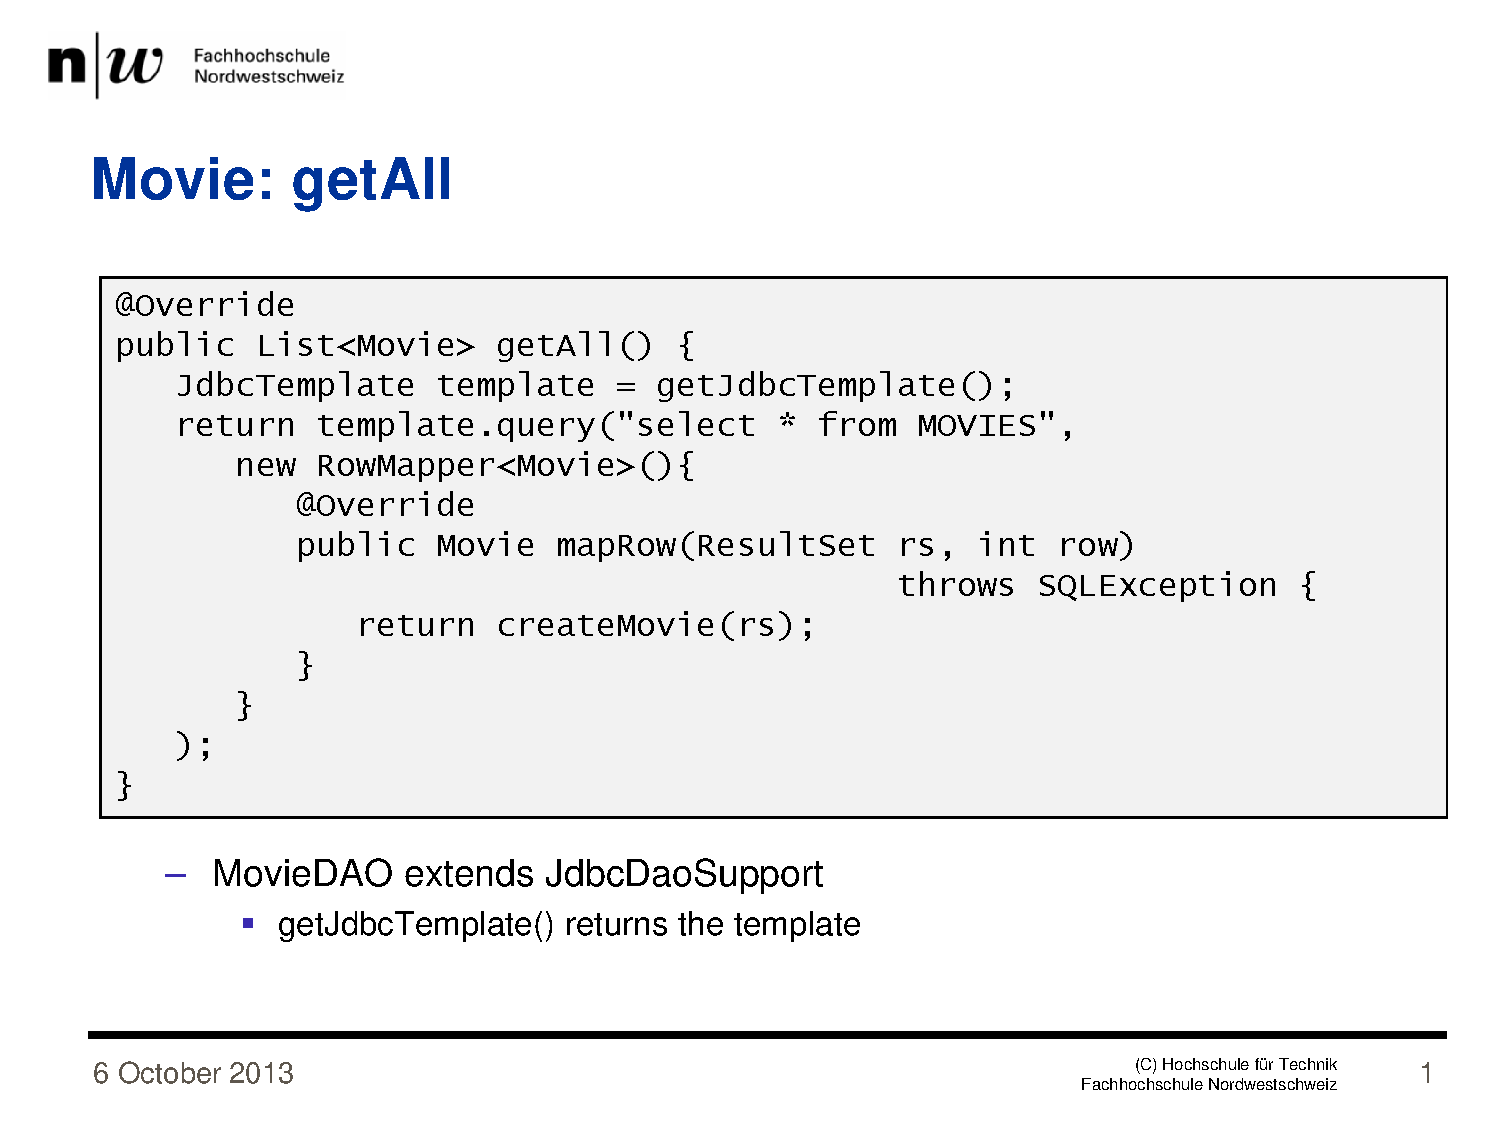
\includepdf[pages=-,nup=2x2]{d1.pdf}
\section{JPA}
 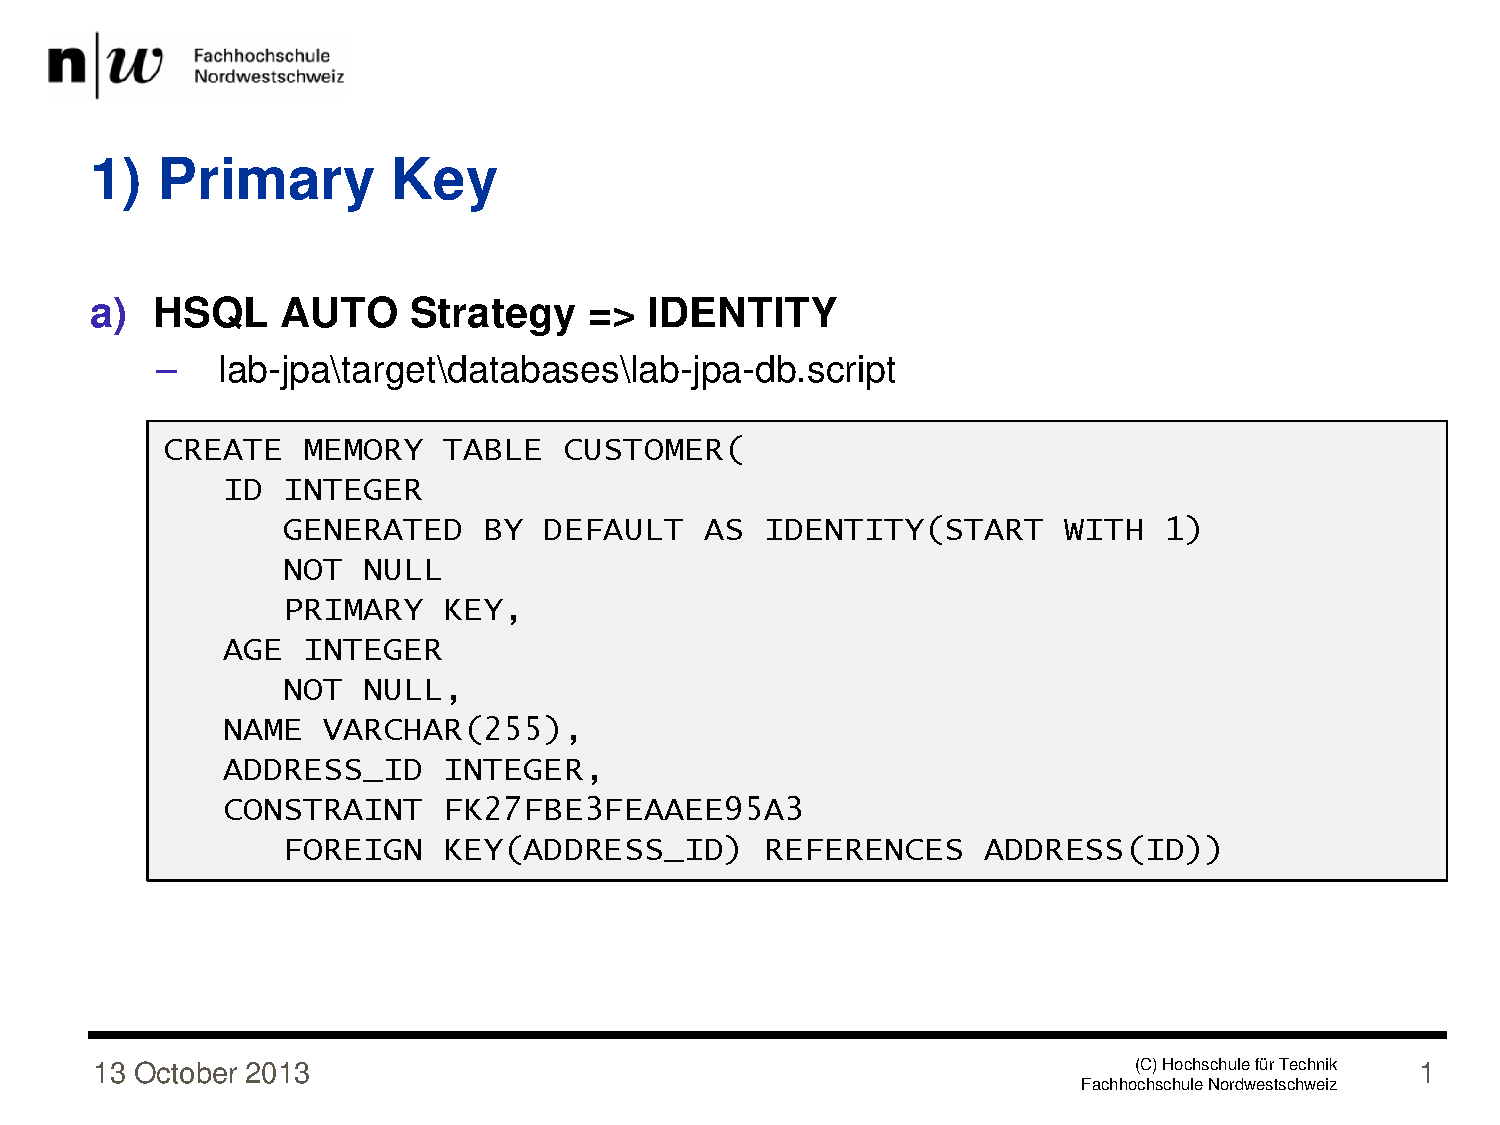
\includepdf[pages=-,nup=2x2]{d2.pdf}
  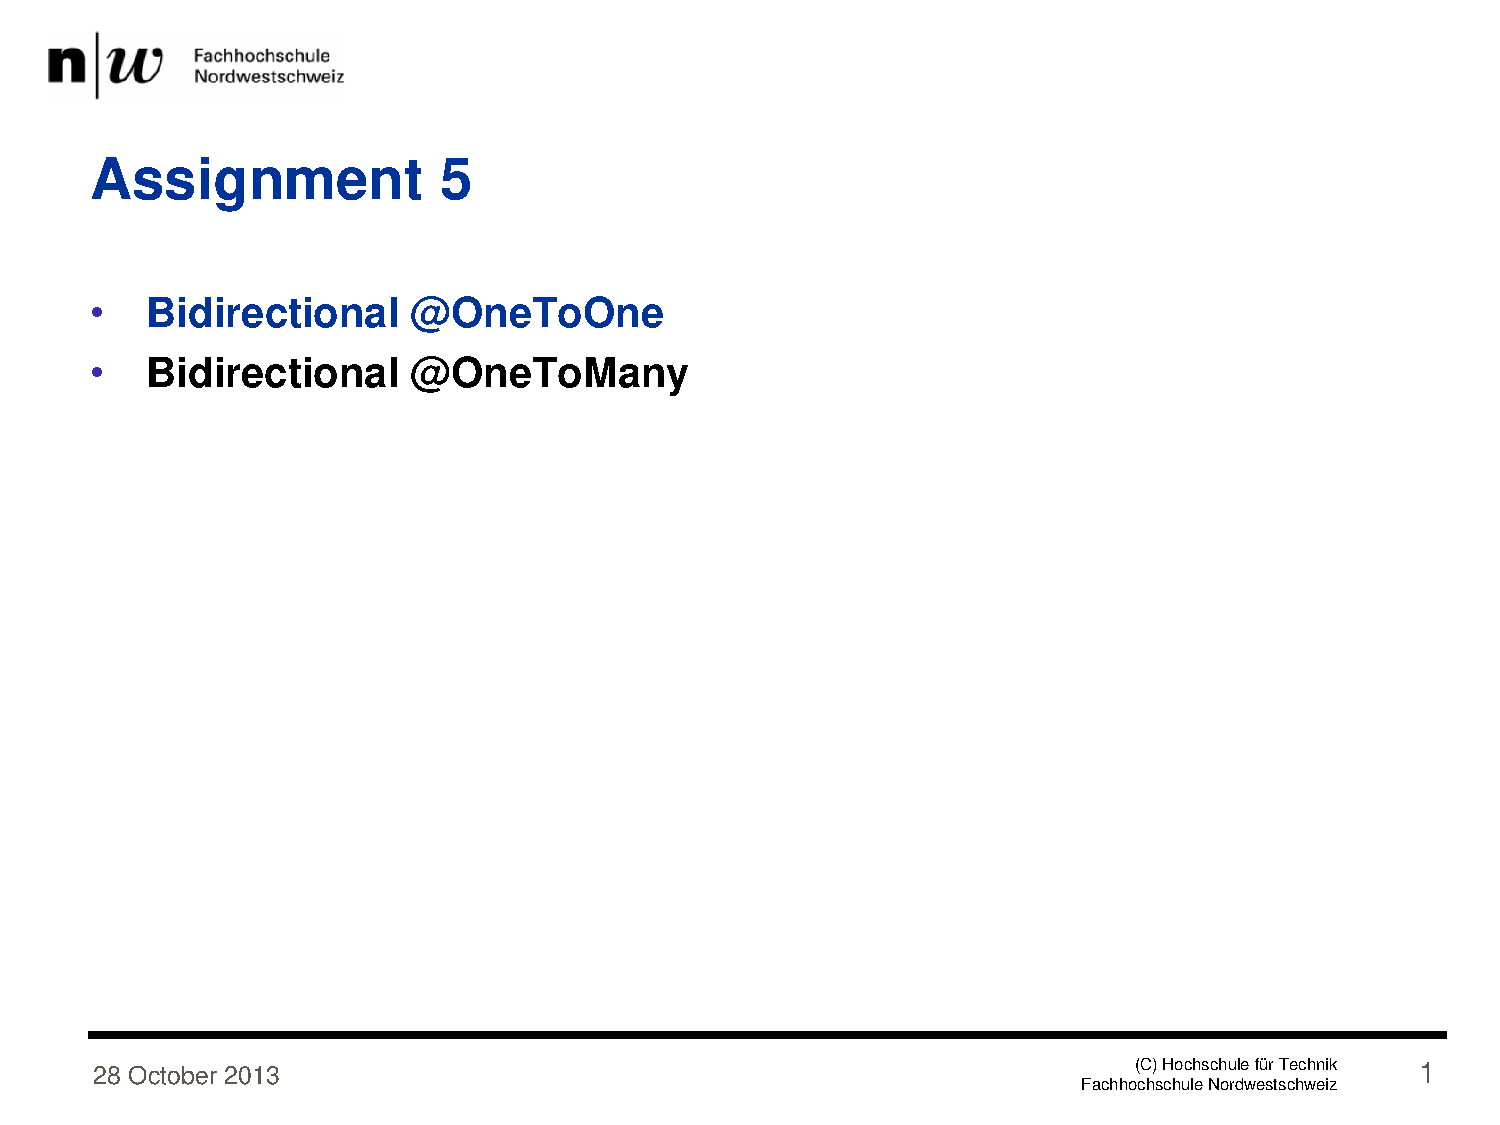
\includepdf[pages=-,nup=2x2]{d3.pdf}
\chapter{Caching, Email, Sheduled Tasks, Docker, RESTTest}
 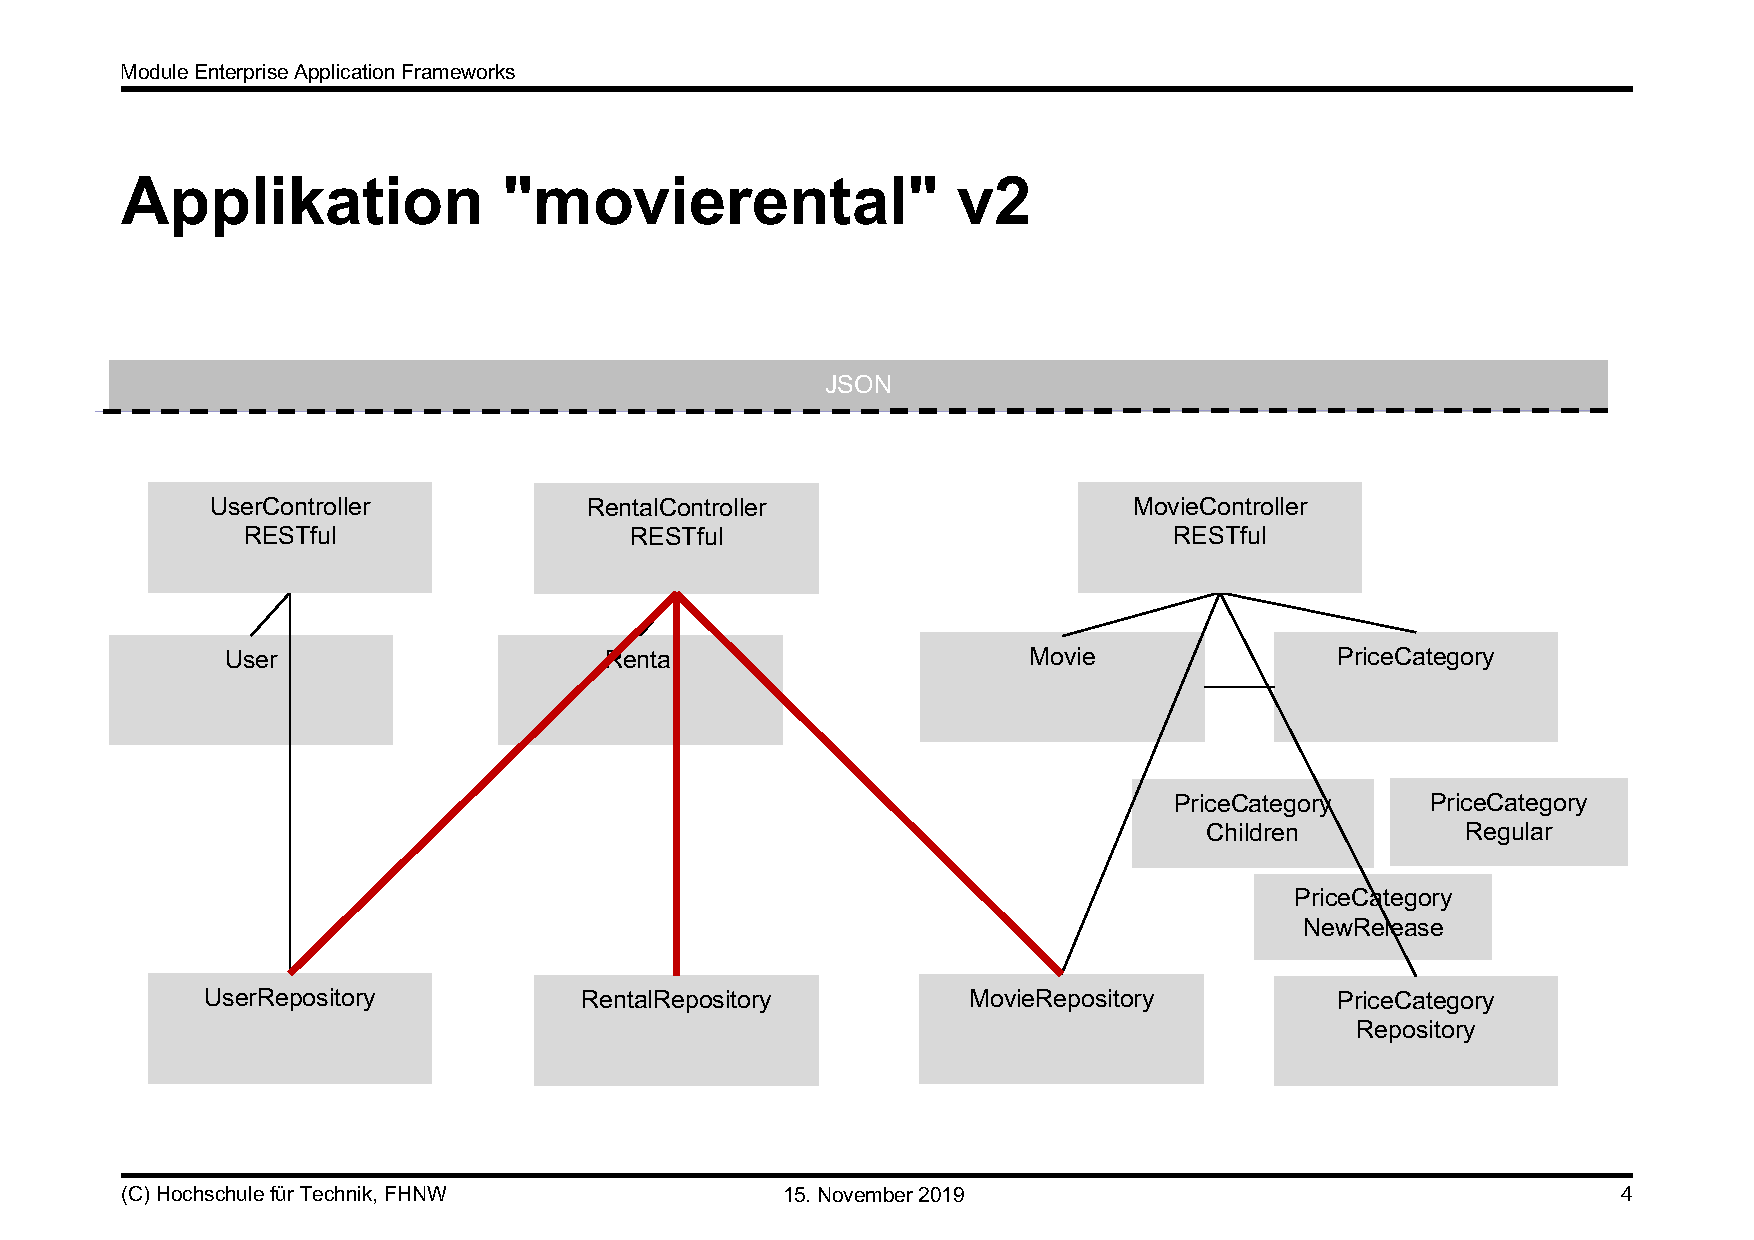
\includepdf[pages=-,nup=2x2]{cache.pdf}
 
\chapter{AOP}
 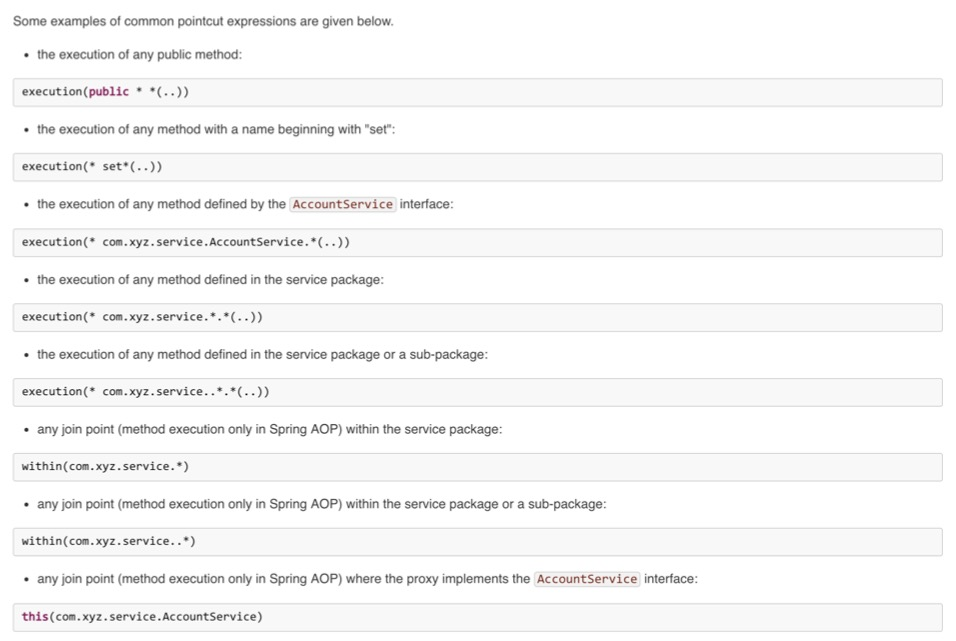
\includegraphics[scale=0.4,keepaspectratio=true]{aop_ex.jpeg}
\begin{lstlisting}[caption=Aspekt Beispiele]
 @Aspect
@Component
public class MovieProgressAspect {
	private static final Logger LOG = LoggerFactory
			.getLogger(MovieProgressAspect.class);

	@Autowired
	private MovieProgress movieProgress;

	@AfterReturning(pointcut = "execution(* ch.fhnw.edu.rental.services.MovieService.getAllMovies())", returning = 
"movielist")
	public void checkMovieList(List<Movie> movielist) {
		if (movieProgress.checkForUpdateProgress(movielist)) {
			LOG.debug(movieProgress.toString());
		}
	}
}

@Aspect
@Component
public class MovieStatisticAspect {
    private static final Logger LOG = LoggerFactory.getLogger(MovieStatisticAspect.class);
    @Autowired
    private MovieStatistic statistic;

    @Around("execution(* *..*.MovieService.saveOrUpdateMovie(..)) && args(movie)")
    public void checkSave(ProceedingJoinPoint pjp, Movie movie) throws Throwable  {
	    if (movie.getId() == null) {
	    	pjp.proceed();
	    	statistic.movieAdded();
	    	LOG.debug("Actual # of movies are {}", statistic.getNrOfMovieInstance());
    	} else {
    		pjp.proceed();
    	}
    }
    
    
    
    @After("execution(* *..*.MovieService.deleteMovie(..))")
    public void checkDelete()  {
    	statistic.movieDeleted();
    	LOG.debug("Actual # of movies are {}", statistic.getNrOfMovieInstance());
    }    
}

@Aspect
@Component
public class MovieValidatorAspect {
	private static final Logger LOG = LoggerFactory
			.getLogger(MovieValidatorAspect.class);
	@Autowired
	private MovieValidator movieValidator;

	@Around("execution(* *..*.MovieService.saveOrUpdateMovie(..)) && args(movie)")
	public void checkMovieEntity(ProceedingJoinPoint pjp, Movie movie) throws Throwable {
		if (movieValidator.isValid(movie)) {
			LOG.debug("Proceeding for movie '{}'", movie.getTitle());
			pjp.proceed();
		} else {
			LOG.debug("Movie '{}' is not valid", movie.getTitle());
			throw new RuntimeException("Movie Bean not valid");
		}
	}
}
\end{lstlisting}
\begin{lstlisting}[caption=SwaggerConfig.java]
package ch.fhnw.edu.eaf.movierental;

import org.springframework.context.annotation.Bean;
import org.springframework.context.annotation.Configuration;

import springfox.documentation.builders.PathSelectors;
import springfox.documentation.builders.RequestHandlerSelectors;
import springfox.documentation.spi.DocumentationType;
import springfox.documentation.spring.web.plugins.Docket;
import springfox.documentation.swagger2.annotations.EnableSwagger2;

// Needs in build.gradle dependencies
//  implementation 'io.springfox:springfox-swagger2:2.9.2'
//  implementation 'io.springfox:springfox-swagger-ui:2.9.2'

@Configuration
@EnableSwagger2
public class SwaggerConfig {                                    
    @Bean
    public Docket api() { 
        return new Docket(DocumentationType.SWAGGER_2)  
          .select()                                  
          .apis(RequestHandlerSelectors.any())              
          .paths(PathSelectors.any())                          
          .build();                                           
    }
}
\end{lstlisting}
\chapter{Convention over Configuration}
\section{Main Code}
\begin{lstlisting}[caption=HelloWorldConfiguration.java]	
package ch.fhnw.edu.eaf.app;

import org.springframework.boot.autoconfigure.SpringBootApplication;
import org.springframework.context.annotation.ComponentScan;
import org.springframework.context.annotation.Configuration;
import org.springframework.context.annotation.PropertySource;

// Use this annotations for java config. They can be commented out if using spring boot conventions
@Configuration
@ComponentScan(basePackages = {"ch.fhnw.edu.eaf.app.domain"})
@PropertySource(value={"classpath:application.properties"})
// Use this annotation to fire spring boot conventions
@SpringBootApplication
public class HelloWorldConfiguration {
}
\end{lstlisting}
\begin{lstlisting}[caption=HelloWorldConfigurationWithoutConfiguration.java]
package ch.fhnw.edu.eaf.app;

import org.springframework.context.annotation.Bean;
import org.springframework.context.annotation.Configuration;
import org.springframework.context.annotation.PropertySource;

import ch.fhnw.edu.eaf.app.domain.MessageProvider;
import ch.fhnw.edu.eaf.app.domain.MessageRenderer;
import ch.fhnw.edu.eaf.app.domain.impl.ExternalizedHelloWorldMessageProvider;
import ch.fhnw.edu.eaf.app.domain.impl.StandardOutRenderer;

@Configuration
@PropertySource(value={"classpath:application.properties"})
public class HelloWorldConfigurationWithoutComponentScan {
    @Bean
    public MessageProvider messageProvider() {
        return new ExternalizedHelloWorldMessageProvider();
    }

    @Bean
    public MessageRenderer messageRenderer() {
        MessageRenderer renderer = new StandardOutRenderer();
        renderer.setMessageProvider(messageProvider());
        return renderer;
    }
}
	
\end{lstlisting}
\section{XML Configuration}
\begin{lstlisting}[caption=helloConfigWithAnnotationFormat.xml]
<?xml version="1.0" encoding="UTF-8"?>
<beans xmlns="http://www.springframework.org/schema/beans"
	xmlns:xsi="http://www.w3.org/2001/XMLSchema-instance"
	xmlns:context="http://www.springframework.org/schema/context"
	xsi:schemaLocation="http://www.springframework.org/schema/beans http://www.springframework.org/schema/beans/spring-beans-3.1.xsd
		http://www.springframework.org/schema/context http://www.springframework.org/schema/context/spring-context-3.1.xsd">
			
	<!-- load property resources -->
	<context:property-placeholder location="classpath:application.properties"/>
	
	<!-- autodetect spring beans and register them -->
	<context:component-scan base-package="ch.fhnw.edu.eaf.app.domain"/>
</beans>	
\end{lstlisting}

\begin{lstlisting}[caption="helloConfigWithApplicationContextWithXmlFormat.xml]
	<?xml version="1.0" encoding="UTF-8"?>
<beans xmlns="http://www.springframework.org/schema/beans"
	xmlns:context="http://www.springframework.org/schema/context"
	xmlns:xsi="http://www.w3.org/2001/XMLSchema-instance"
	xsi:schemaLocation="http://www.springframework.org/schema/beans http://www.springframework.org/schema/beans/spring-beans-3.1.xsd
		http://www.springframework.org/schema/context http://www.springframework.org/schema/context/spring-context-3.1.xsd">

	<!-- load property resources -->
	<context:property-placeholder location="classpath:application.properties"/>

	<bean id="renderer" class="ch.fhnw.edu.eaf.app.domain.impl.StandardOutRenderer">
		<property name="messageProvider" ref="provider"/>
	</bean>

	<bean id="provider" class="ch.fhnw.edu.eaf.app.domain.impl.ExternalizedHelloWorldMessageProvider">
		<property name="message" value="${helloworld.message}"/>
	</bean>
</beans>
\end{lstlisting}

\section{Tests}
\begin{lstlisting}[caption=HelloWorldAnnotationTest.java]
package ch.fhnw.edu.eaf.app;

import static org.junit.Assert.assertEquals;
import static org.junit.Assert.assertNotNull;

import org.junit.Test;
import org.junit.runner.RunWith;
import org.springframework.beans.factory.annotation.Autowired;
import org.springframework.test.context.ContextConfiguration;
import org.springframework.test.context.junit4.SpringRunner;

import ch.fhnw.edu.eaf.app.domain.MessageProvider;
import ch.fhnw.edu.eaf.app.domain.MessageRenderer;

@RunWith(SpringRunner.class)
@ContextConfiguration(locations = {"/spring/helloConfigWithAnnotationFormat.xml"})
public class HelloWorldAnnotationTest {
	
	@Autowired
	private MessageProvider messageProvider;
	
	@Autowired
	private MessageRenderer messageRenderer;
	
	@Test
	public void testGetMessage() {
		assertEquals("Herzlich willkommen!", messageProvider.getMessage());
	}

	@Test
	public void testGetMessageProvider() {
		assertNotNull(messageRenderer.getMessageProvider());
	}
}
\end{lstlisting}


\begin{lstlisting}[caption=HelloWorldConventionTest.java]
package ch.fhnw.edu.eaf.app;

import static org.junit.Assert.assertEquals;
import static org.junit.Assert.assertNotNull;

import org.junit.Test;
import org.junit.runner.RunWith;
import org.springframework.beans.factory.annotation.Autowired;
import org.springframework.boot.test.context.SpringBootTest;
import org.springframework.test.context.junit4.SpringRunner;

import ch.fhnw.edu.eaf.app.domain.MessageProvider;
import ch.fhnw.edu.eaf.app.domain.MessageRenderer;

@RunWith(SpringRunner.class)
// SpringBootTest searches for a class annotated with @SpringBootConfiguration
@SpringBootTest
public class HelloWorldConventionTest {
	
	@Autowired
	private MessageProvider messageProvider;
	
	@Autowired
	private MessageRenderer messageRenderer;
	
	@Test
	public void testGetMessage() {
		assertEquals("Herzlich willkommen!", messageProvider.getMessage());
	}

	@Test
	public void testGetMessageProvider() {
		assertNotNull(messageRenderer.getMessageProvider());
	}

}

\end{lstlisting}

\begin{lstlisting}[caption=HelloWorldJavaTest.java]
package ch.fhnw.edu.eaf.app;

import static org.junit.Assert.assertEquals;
import static org.junit.Assert.assertNotNull;

import org.junit.Test;
import org.junit.runner.RunWith;
import org.springframework.beans.factory.annotation.Autowired;
import org.springframework.test.context.ContextConfiguration;
import org.springframework.test.context.junit4.SpringRunner;

import ch.fhnw.edu.eaf.app.domain.MessageProvider;
import ch.fhnw.edu.eaf.app.domain.MessageRenderer;

@RunWith(SpringRunner.class)
@ContextConfiguration(classes= {ch.fhnw.edu.eaf.app.HelloWorldConfiguration.class})
public class HelloWorldJavaTest {
	
	@Autowired
	private MessageProvider messageProvider;
	
	@Autowired
	private MessageRenderer messageRenderer;
	
	@Test
	public void testGetMessage() {
		assertEquals("Herzlich willkommen!", messageProvider.getMessage());
	}

	@Test
	public void testGetMessageProvider() {
		assertNotNull(messageRenderer.getMessageProvider());
	}
}

\end{lstlisting}

\begin{lstlisting}[caption=HelloWorldJavaTestWithoutComponentScan.java]
package ch.fhnw.edu.eaf.app;

import static org.junit.Assert.assertEquals;
import static org.junit.Assert.assertNotNull;

import org.junit.Test;
import org.junit.runner.RunWith;
import org.springframework.beans.factory.annotation.Autowired;
import org.springframework.test.context.ContextConfiguration;
import org.springframework.test.context.junit4.SpringRunner;

import ch.fhnw.edu.eaf.app.domain.MessageProvider;
import ch.fhnw.edu.eaf.app.domain.MessageRenderer;

@RunWith(SpringRunner.class)
@ContextConfiguration(classes= {HelloWorldConfigurationWithoutComponentScan.class})
public class HelloWorldJavaTestWithoutComponentScan {
	
	@Autowired
	private MessageProvider messageProvider;
	
	@Autowired
	private MessageRenderer messageRenderer;
	
	@Test
	public void testGetMessage() {
		assertEquals("Herzlich willkommen!", messageProvider.getMessage());
	}

	@Test
	public void testGetMessageProvider() {
		assertNotNull(messageRenderer.getMessageProvider());
	}
}

\end{lstlisting}
\begin{lstlisting}[caption=HelloWorldXMLTest.java]
package ch.fhnw.edu.eaf.app;

import static org.junit.Assert.assertEquals;
import static org.junit.Assert.assertNotNull;

import org.junit.Test;
import org.junit.runner.RunWith;
import org.springframework.beans.factory.annotation.Autowired;
import org.springframework.test.context.ContextConfiguration;
import org.springframework.test.context.junit4.SpringRunner;

import ch.fhnw.edu.eaf.app.domain.MessageProvider;
import ch.fhnw.edu.eaf.app.domain.MessageRenderer;

@RunWith(SpringRunner.class)
@ContextConfiguration(locations = {"/spring/helloConfigWithApplicationContextWithXmlFormat.xml"})
public class HelloWorldXMLTest {
	
	@Autowired
	private MessageProvider messageProvider;
	
	@Autowired
	private MessageRenderer messageRenderer;
	
	@Test
	public void testGetMessage() {
		assertEquals("Herzlich willkommen!", messageProvider.getMessage());
	}

	@Test
	public void testGetMessageProvider() {
		assertNotNull(messageRenderer.getMessageProvider());
	}
}

\end{lstlisting}
\end{document}